
\lstset{
     literate=%
         {á}{{\'a}}1
         {í}{{\'i}}1
         {é}{{\'e}}1
         {ý}{{\'y}}1
         {ú}{{\'u}}1
         {ó}{{\'o}}1
         {ě}{{\v{e}}}1
         {š}{{\v{s}}}1
         {č}{{\v{c}}}1
         {ř}{{\v{r}}}1
         {ž}{{\v{z}}}1
         {ď}{{\v{d}}}1
         {ť}{{\v{t}}}1
         {ň}{{\v{n}}}1                
         {ů}{{\r{u}}}1
         {Á}{{\'A}}1
         {Í}{{\'I}}1
         {É}{{\'E}}1
         {Ý}{{\'Y}}1
         {Ú}{{\'U}}1
         {Ó}{{\'O}}1
         {Ě}{{\v{E}}}1
         {Š}{{\v{S}}}1
         {Č}{{\v{C}}}1
         {Ř}{{\v{R}}}1
         {Ž}{{\v{Z}}}1
         {Ď}{{\v{D}}}1
         {Ť}{{\v{T}}}1
         {Ň}{{\v{N}}}1                
         {Ů}{{\r{U}}}1    
}

\chapter{Úvod}
Úlohou tejto práce je vytvoriť aplikáciu na tvorbu parametrických 3D modelov. Tieto modely sú tvorené pomocou geometrických operácii. Aplikácia by mala umožňovať prácu pomocou dvoch rozhraní, grafického a programátorského. Grafické rozhranie musí umožniť návrhárovi jednoduchú tvorbu modelov. Programátorské rozhranie umožní používať  Hodnota u parametrov sa dá ľubovolne meniť  

Druhá kapitola sa zaoberá parametrickými modelmi, ich tvorbou a ich históriou. V tejto kapitole tiež popisujem existujúce programy pre tvorbu parametrických modelov.

Tretia kapitola sa zaoberá štruktúrami pre objekty.

V štvrtej kapitole je výpis použitých geometrických operácii. Tieto operácie sú rozdelené na štyri druhy, podľa toho aký typ objektu vytvárajú. Sú to bodové geometrické operácie, úsečkové, plošné a objemové. U jednotlivých geometrických operácii je uvedené ako dané objekty vytvárajú, parametre ktoré jednotlivé operácie potrebujú a formát zápisu, ktorý sa používa na ich vytvorenie a v ktorom sa tiež ukladajú. Parametre typu $Float$ (desatinné čísla) je možné pomenovať, a tak na ne vytvoriť odkaz pre nastavovanie parametrov. 

V piatej kapitole je opísané grafické užívateľské rozhranie, ktoré umožňuje jednoduchý návrh geometrických modelov. Grafické užívateľské rozhranie umožňuje pridanie, vloženie, úpravu aj zmazanie použitých geometrických operácii a pri geometrickej operácii ktorá má ako parameter nedostupný objekt (bol presunutý alebo odstránený), upozorní užívateľa. Grafické užívateľské rozhranie pozostáva z dvoch okien. Jedno pre správu geometrických operácii, zobrazenie orientovaného grafu, ktorý operácie tvoria a samotné vykresľovanie modelu pomocou OpenGL a druhé dialógové okno na výber geometrickej operácie a nastavovanie jej parametrov. 

\chapter{Parametrické 3d modely}
Typickým návrhovým médiom je ceruzka a papier. Presnejšie ceruzka, guma a papier. Ceruzka pridáva a guma odoberá. Po pridaní niekoľkých nástrojov, ako pravítko, kružidlo a uhlomer sa kresby stanú presnejšími a precíznejšími modelmi navrhovanej idei. Dizajnéri musia pridávať a odoberať značky a spájať ich \cite{woodbury2010elements}.

Konvenčné návrhové systémy fungujú práve na tomto princípe. Parametrické modelovanie predstavuje zásadnú zmenu. Značky ktoré sú základom návrhu spolu súvisia a vzájomne menia svoju pozíciu. Dizajnéri už nemusia iba pridávať a odoberať, ale môžu vytvárať medzi bodmi vzťahy a upravovať model, aby aj po zmazaní, časti závisiace od zmazaných častí mohli závisieť od častí ktoré zostali \cite{woodbury2010elements}. 

Vďaka tomu, že sú parametrické modely vytvárané pomocou geometrických operácii. Keďže operácie sú závislé na výsledku inej operácie, pri zmene niektorého z parametrov je potrebné model znova vytvoriť. Pre skrátenie času pre vytvorenie operácie je možné upravovať len operácie, ktoré boli touto zmenou dotknuté.


\todo{TODO}\\
https://onlinelibrary.wiley.com/doi/pdf/10.1002/ad.2019\\
https://onlinelibrary.wiley.com/doi/epdf/10.1002/ad.2020\\


%https://en.wikipedia.org/wiki/Parametric_design#cite_note-Frazer-3
%https://en.wikipedia.org/wiki/Antoni_Gaud%C3%AD



\section{História parametrických modelov}
Pôvod slova \texts{parameter} pochádza z matematiky, kde popisuje matematickú metódu, ktorá používa nezávislé premenné, zvané parametre. Debatuje sa ale ohľadom toho, kedy začali dizajnéry používať toto slovo \cite{davis_2013}. David Gerber v svojej doktorskej práci \textit{Parametric Practice} (2007) pripisoval Maurice Reiter prvé použitie tohoto slova na papieri s názvom \textit{Parametric Design} z roku 1988. V roku 1988 bol tiež vydaný prvý komerčne úspečný softvér pre parametrické modelovanie \textsf{Pro/ENGINEER} firmou Parametric Technology Corporation založenou matematikom Samuelom Geisbergom v roku 1985.

Robert Stiles ale dokázal, že skutočný pôvod tohoto slova bol už o niekoľko dekád skôr pomocou zápisov architekta Luigi Morettiho z rokov 1940.  Moretti písal o parametrickej architektúre, ktorú definoval ako architektonické systémy s cieľom 
definovať vzťahy medzi rozmermi závislými od rôznych parametrov.
Moretti v roku 1960 použil ako príklad dizajn štadióna \ref{fig:morretiStadion}, kde vysvetlil, ako sa môže štadión meniť pomocou devätnástich parametrov, ktoré zahŕňali pozorovacie uhli a cenové náklady na betón. Tento model vytvoril už za pomoci počítača 610 od spoločnosti IBM\cite{doi:10.1002/ad.2019}. O pár rokov neskôr Moretti navrhol Watergate Complex \ref{fig:Watergate}, ktorý je prvou veľkou stavebnou prácou na ktorú boli využité počítače \cite{davis_2013}. 


\afterpage{
\begin{figure}[H]
    \centering
    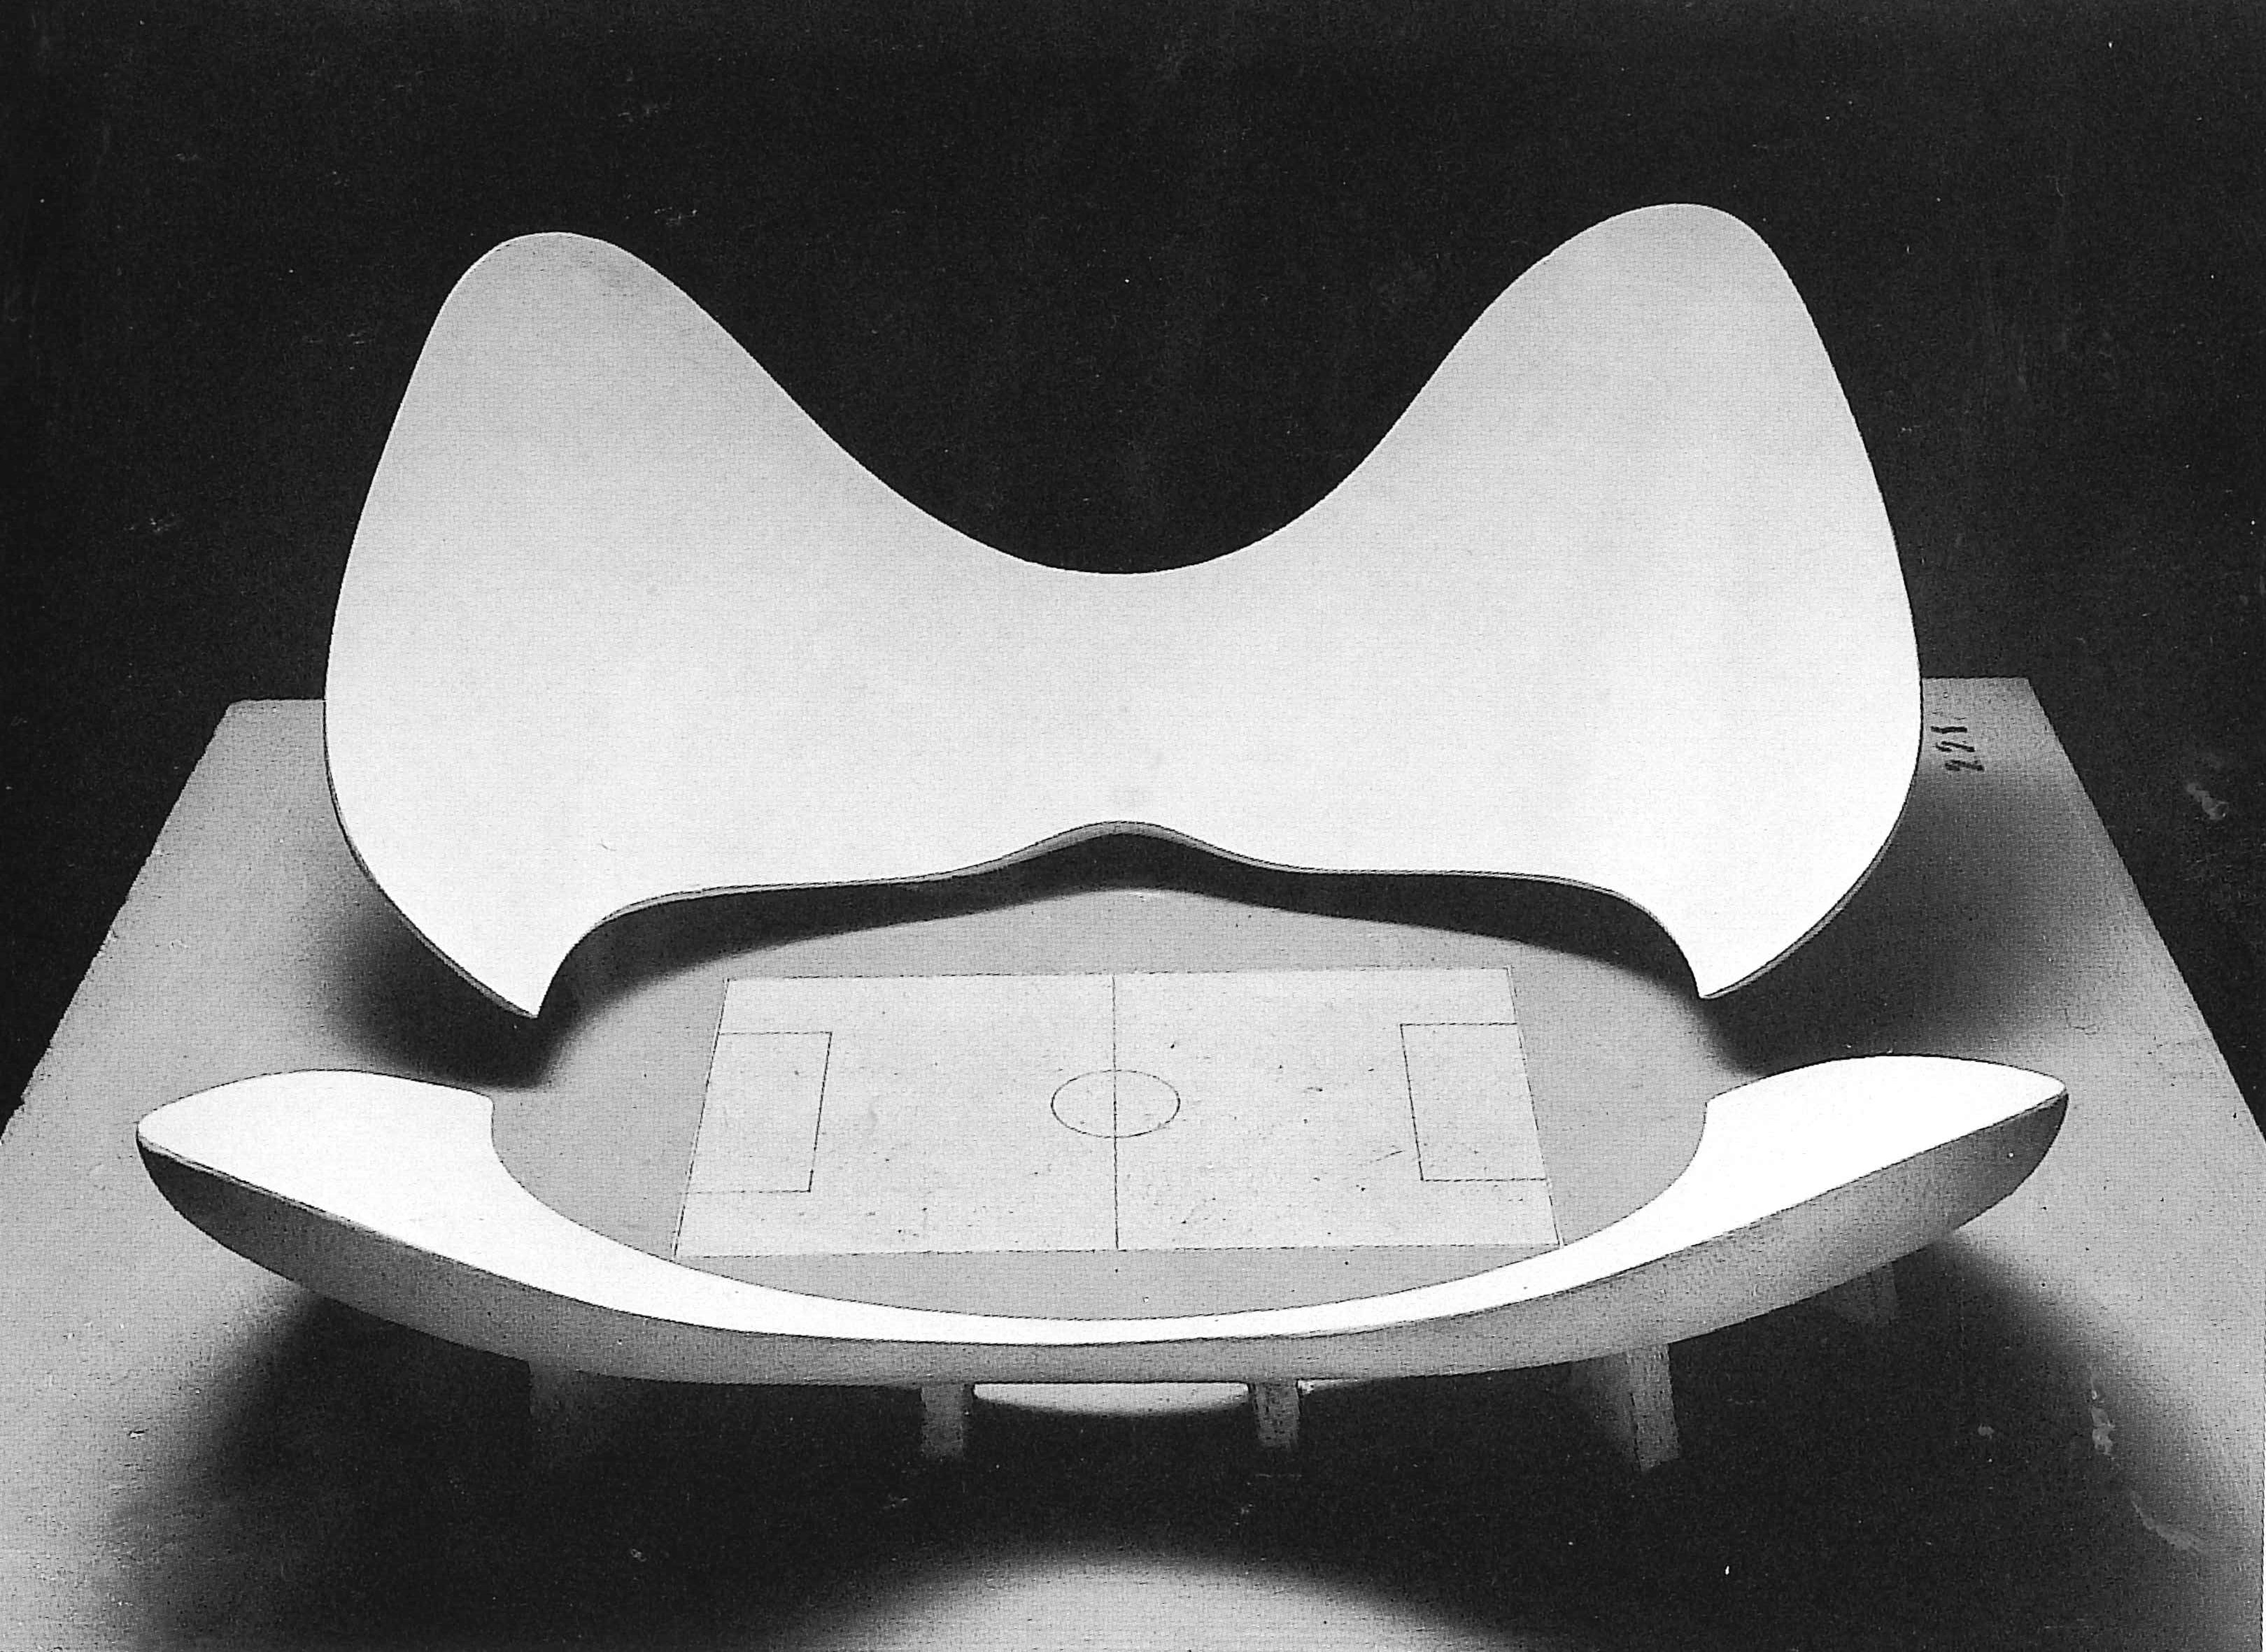
\includegraphics[width = \linewidth]{obrazky-figures/moretti_1.jpg}
    \caption{Model štadióna N od Luigi Moretti. Tento model bol vystavený na výstave parametrickej architektúry v Twelfth Milan Triennial v roku 1960. Parametrický model pozostávajúci z devätnástich parametrov. Zdroj:  \footnotemark}
    \label{fig:morretiStadion}
\end{figure}
\footnotetext{http://www.danieldavis.com/thesis-ch2/}

}

\afterpage{
\begin{figure}[H]
    \centering
    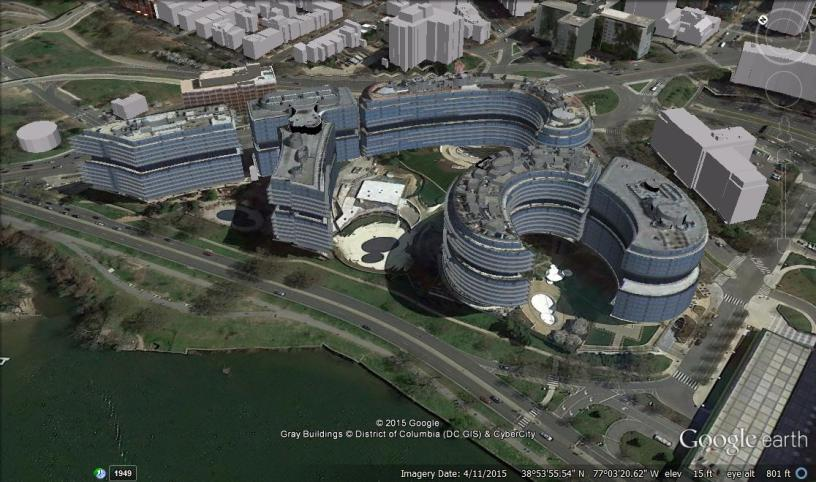
\includegraphics[width = \linewidth]{obrazky-figures/watergate-complex.jpg}
    \caption{Watergate Complex navrhnutý Luigi Morettim. Prvý veľký stavebný projekt, na ktorý boli využité parametrické modely. Zdroj: \footnotemark}
    \label{fig:Watergate}
\end{figure}
\footnotetext{https://seanmunger.com/2015/06/17/earth-the-watergate-complex-famous-for-more-than-just-burglars-and-tapes/}

}









\chapter{Geometrické tvary}
\label{chapt:Geometrické_tvary}
štruktúra objektov \ref{fig:StromDedicnosti}.

\begin{figure}[H]
	\centering
	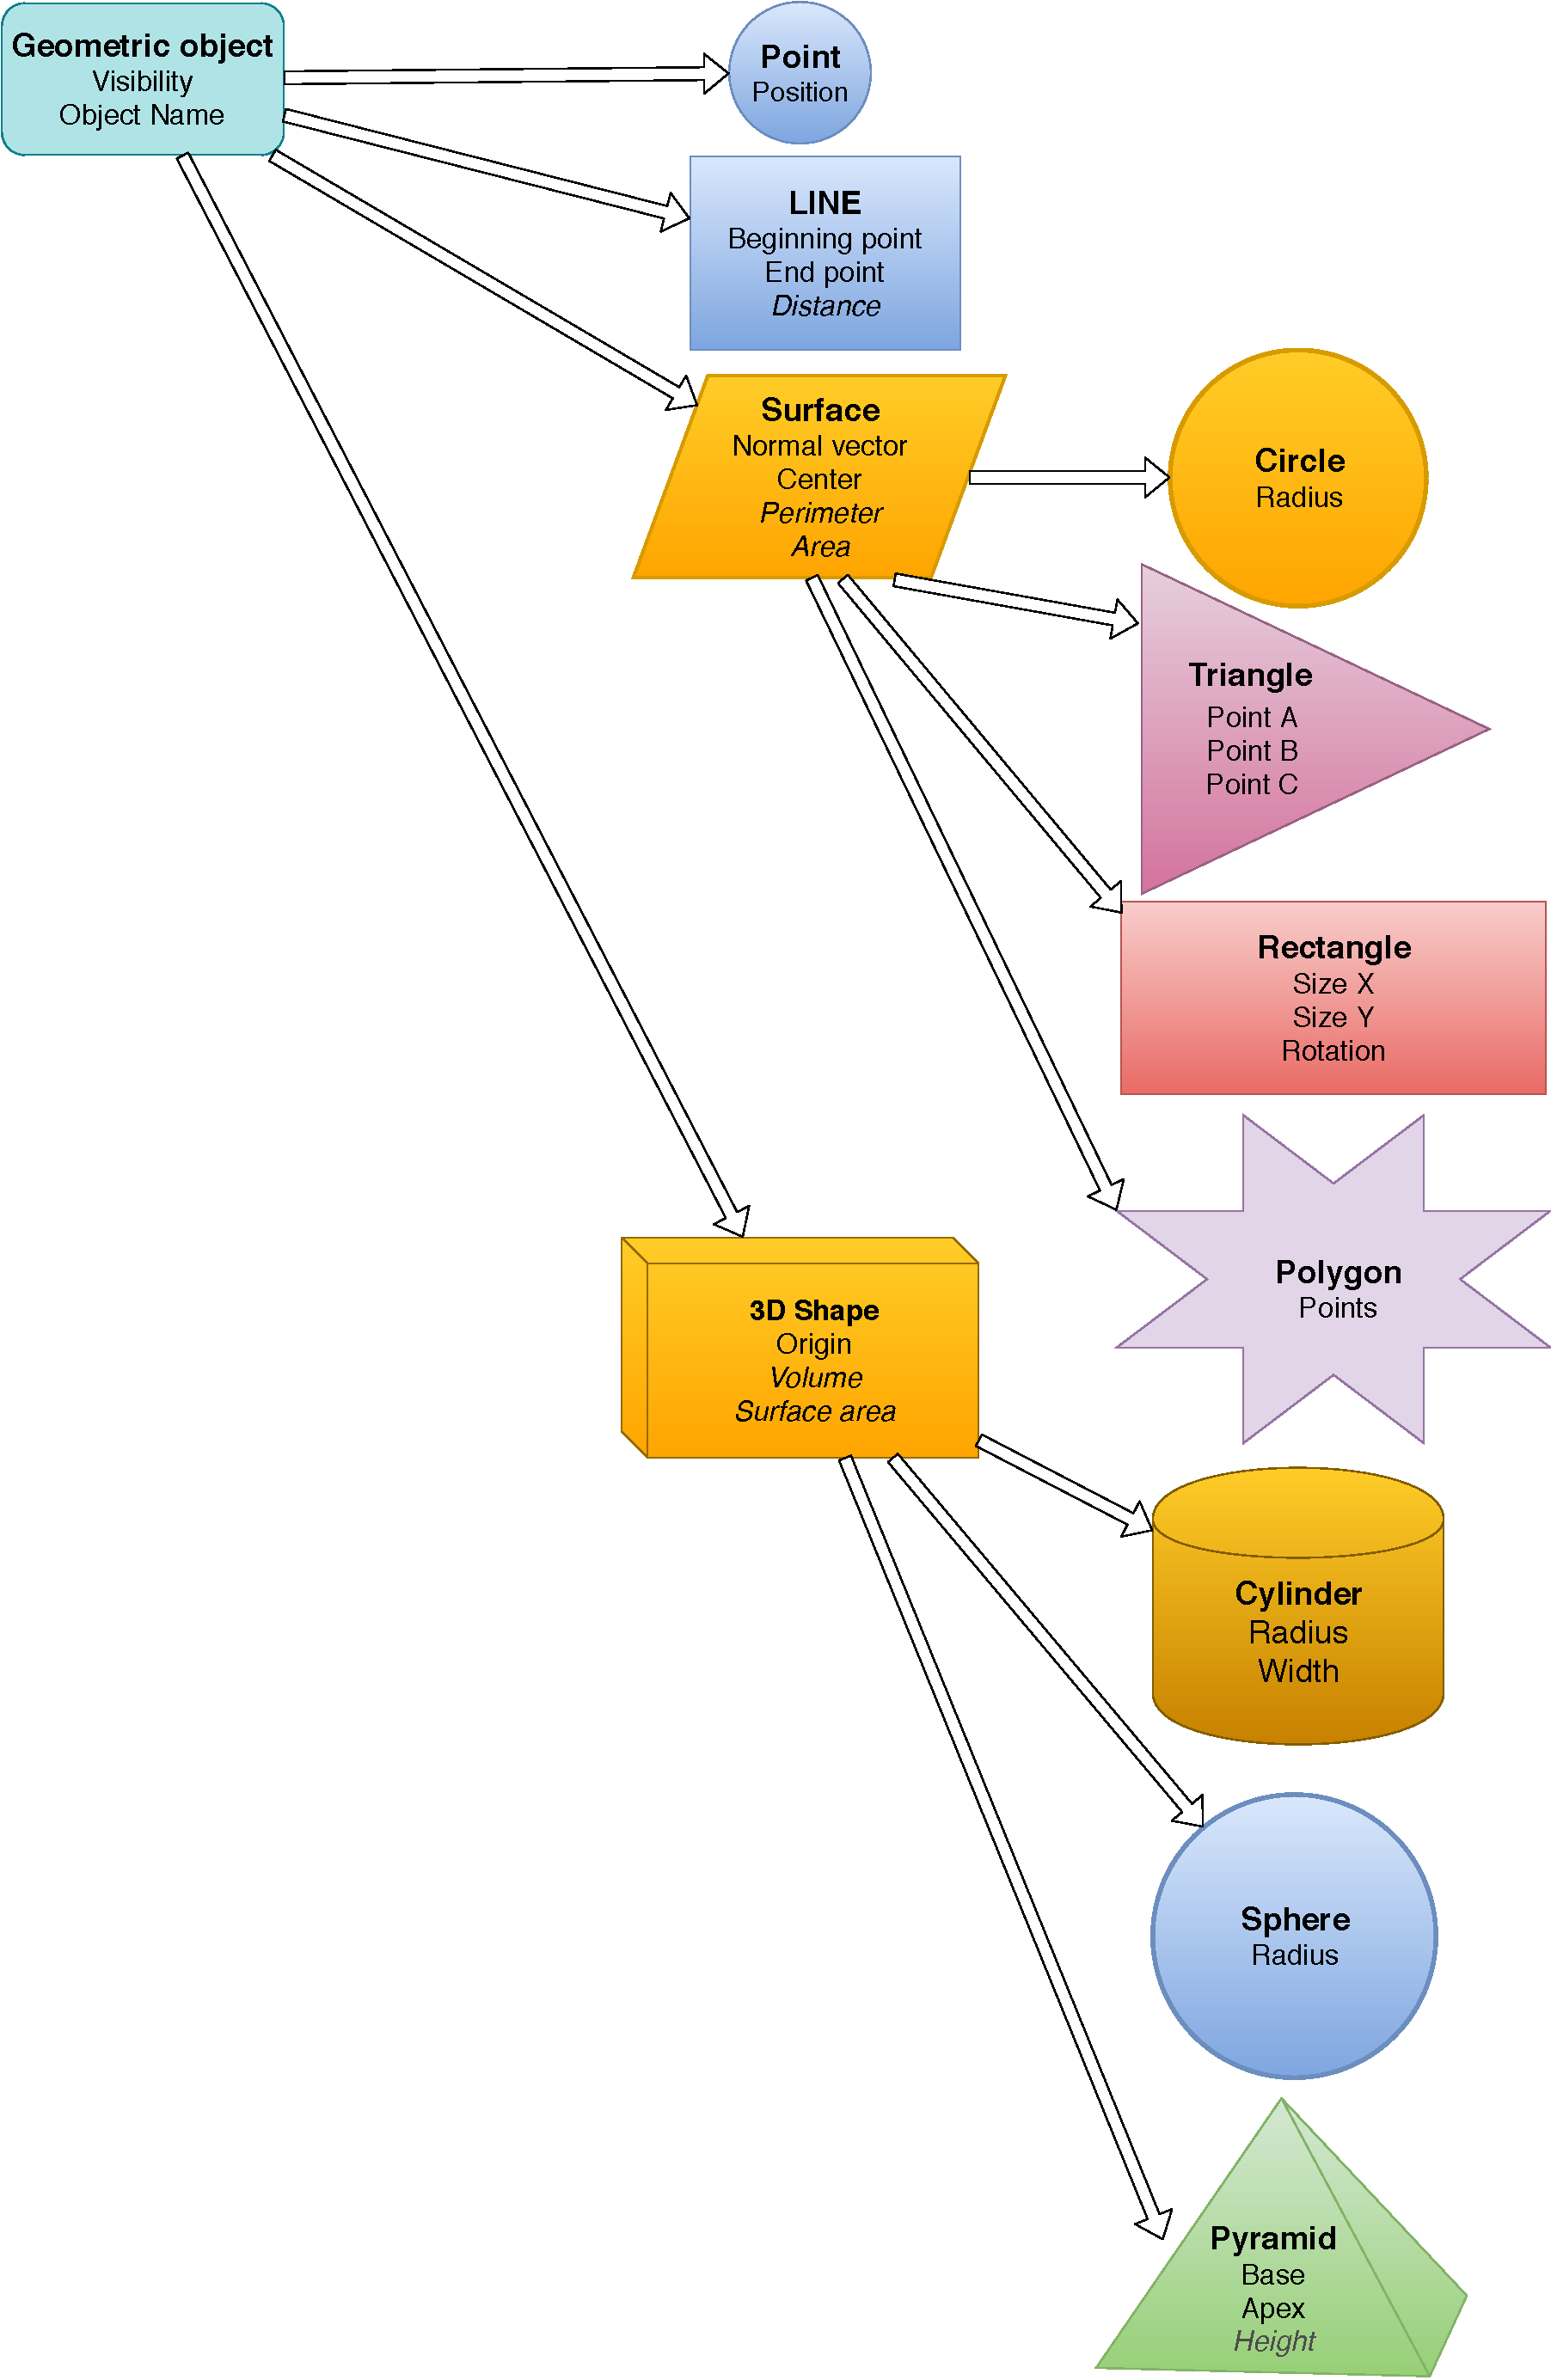
\includegraphics[height=\textheight]{obrazky-figures/Diagram/Draw/DP Navrh operacii-Structure.pdf}
	\caption{Štruktúry objektov vytvárajú strom dedičnosti. Pri každom objekte je uvedené, aké informácie uchovávajú}
	\label{fig:StromDedicnosti}
\end{figure}



\chapter{Geometrické operácie}
Geometrické operácie sa delia na 4 typy podľa toho, aký typ objektu sa dá pomocou nich vytvoriť. Sú to operácie bodové, úsečkové, plošné a priestorové. Na vytváranie zložitejších objektov je potrebné využívať jednoduchšie geometrické objekty. 

Všetky geometrické operácie sa dajú zapisovať pomocou textovej podoby. Tento textový zápis operácii je taktiež uvedený pri jednotlivých operáciach nižšie. 
Textová podoba geometrickej operácie sa začína názvom použitej geometrickej operácie a parametrami uvedenými v zátvorkách ( a ), oddelenými znakom \texttt{','}.  U jednotlivých parametrov sa medzery na začiatku a konci ignorujú.

Pri parametroch typu $Float$ sa požaduje desatinné číslo, pri ostatných parametroch je potrebné uviesť názov existujúceho objektu, ktorý je rovnakého typu alebo podtypu aký je vyžadovaný. Požadované parametre pre jednotlivé geometrické operácie sú uvedené nižšie. 

Parametrom typu $Float$ je možné vytvoriť názov, pomocou ktorého sa bude dať na daný parameter neskôr pristupovať. 
Tento názov sa zadáva za hodnotou parametra oddelený znakom \texttt{';'}.

Jednotlivé operácie sa oddeľujú bodkočiarkou \texttt{';'}. 
Táto textová podoba geometrických operácii sa používa aj pre uloženie do súboru a jeho neskoršie načítanie. 

Pre predstavu ako sa jednotlivé objekty vytvárajú uvádzam príklad pre vytvorenie ihlana s kruhovou podstavou s polomerom 5 a výškou 10:
\begin{itemize}
    \item Na vytvorenie ihlana je potrebné najprv vytvoriť bod na pozícii XYZ, napr. $\left [ 1, 2, 3 \right ]$, ktorý bude slúžiť ako stred kruhovej podstavy.
	\begin{lstlisting}
	Point(bod podstavy, 1, 2, 3 ,0);
	\end{lstlisting}
	\item Na vytvorenie kruhu (podstavy ihlana) je potrebný polomer a normála. Ako normálu, je možné využiť smer ľubovolnej úsečky, ale keďže zatiaľ žiadnu úsečku vytvorenú nemáme, je potrebné ju vytvoriť. Úsečka sa skladá z dvoch bodov a to počiatočného a koncového. Ako normála, sa použije normalizovaný vektor medzi bodom počiatočným a koncovým \ref{eq:normalizacia_usecky}.

	\begin{equation}
		\overrightarrow{normal\_vector}=
		\frac{end\_point - begin\_point}{
		\left \|  end\_point - begin\_point \right \|}
	\label{eq:normalizacia_usecky}
	\end{equation}

	\begin{lstlisting}
	Point(počiatočný bod, 0, 0, 0, 0);
	Point(koncový bod, 1, 1, 1, 0);
	Line(normála, počiatočný bod, koncový bod, 0);
	\end{lstlisting}
	\item Keď už je normála vytvorená, je možné vytvoriť kruh s polomerom 5.
	\begin{lstlisting}
	Circle(podstava, bod podstavy, 5, normála, 0) 
	\end{lstlisting}
	\item Ostáva vytvoriť samotný ihlan s výškou 10.
	\begin{lstlisting}
	Pyramid(ihlan s kruhovou podstavou, podstava, 10, 1)
	\end{lstlisting}
\end{itemize}

\todo{ako vyzerá tento sled operácii pomocou graphviz a v 3D}

Ďalej nasleduje výpis podporovaných geometrických operácii, kde pri každej operácii sa nachádza jednoduchý popis, formát zápisu tejto operácie a grafové zobrazenie vytvorenia tejto operácie.


\section{Bodové operácie}
Bodové operácie sú operácie, ktorých výstupom je bod.
\subsection{Bod}
Základná stavebná jednotka každého objektu. Na vytvorenie bodu je potrebné zadať jeho pozíciu v osiach X, Y a Z. Bod môže byť zadaný buď v absolútnej alebo v relatívnej pozícii, kedy je jeho pozícia závislá na polohe iného bodu.
\begin{lstlisting}
    Point(string name, float X, float Y, float Z,float visibility) 
    Point(string name, float X, float Y, float Z,Point Parent,
        float visibility)
\end{lstlisting}

\begin{figure}[H]
	\centering
	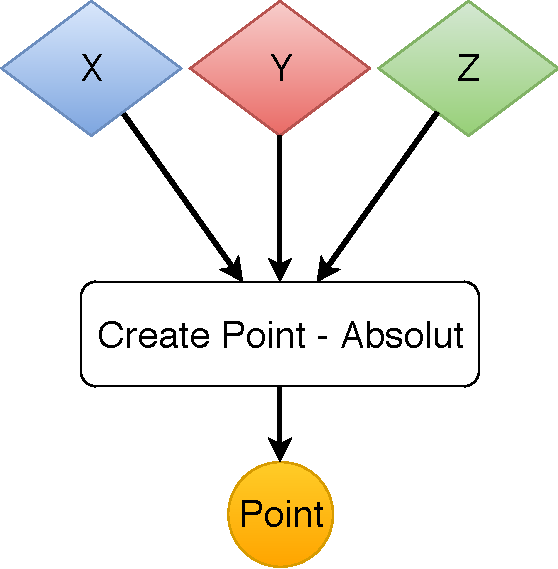
\includegraphics[height=0.3\textwidth]{obrazky-figures/Diagram/Point/DP Navrh operacii-0D - Point.pdf}
	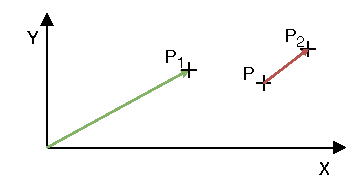
\includegraphics[height=0.3\textwidth]{obrazky-figures/Diagram/Draw/1Points/DP Navrh operacii-0D - Point.pdf}
	\caption{Vytvorenie bodu na absolútnej pozícii}
	\label{fig:1}
\end{figure}
\begin{figure}[H]
	\centering
	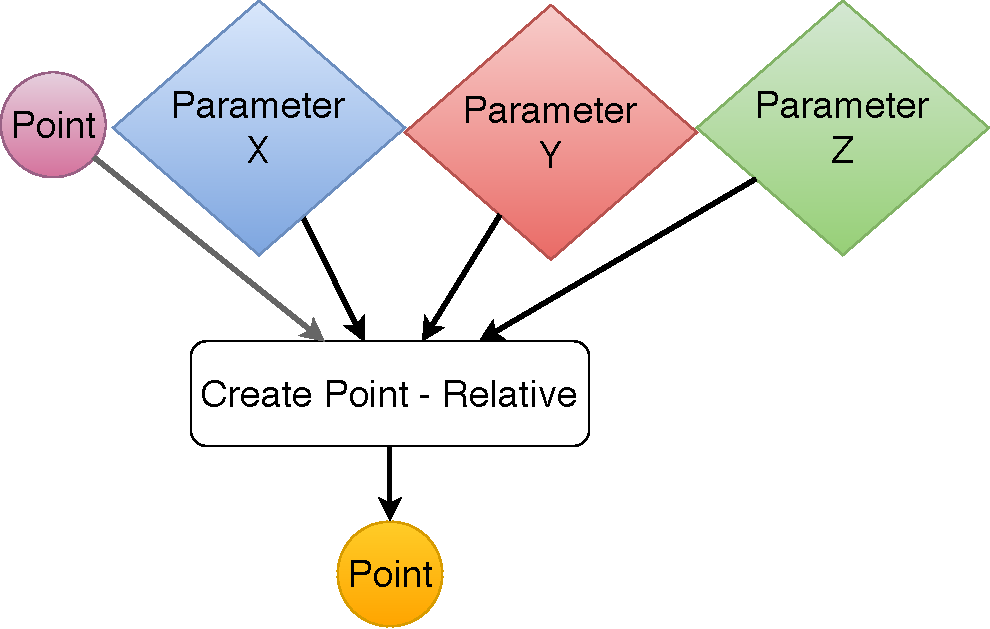
\includegraphics[height=0.3\textwidth]{obrazky-figures/Diagram/Point/DP Navrh operacii-0D - Point2.pdf}
	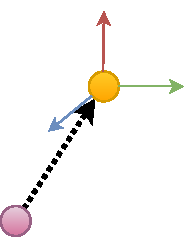
\includegraphics[height=0.3\textwidth]{obrazky-figures/Diagram/Draw/1Points/DP Navrh operacii-0D - PointRelative.pdf}
	\caption{Vytvorenie bodu na relatívnej pozícii od iného bodu}
	\label{fig:1}
\end{figure}

\subsection{Lineárna interpolácia}
Výsledná pozícia bodu závisí od zadanej vzdia\-le\-nos\-ti od počiatočného bodu. Táto vzdia\-le\-nosť môže byť zadaná dĺžkou alebo percentuálne, kde 50\% vytvorí bod uprostred počiatočného a koncového bodu. 
Keďže percentá sa zadávajú tiež vo formáte desatinného čísla ($Float$), bolo potrebné tieto operácie rozlíšiť. Pre zadanie vzdialenosti podľa dĺžky, sa zadáva operácia \texttt{LinearInterpolationDist}, 
pre percentuálnu vzdialenosť je operácia \texttt{LinearInterpolationPerc}.
\begin{lstlisting}
    LinearInterpolationDist(string name, Point fromPoint, Point toPoint,
        float distance, float visibility)
    LinearInterpolationPerc(string name, Point fromPoint, Point toPoint,
        float percentage, float visibility)
\end{lstlisting}


\begin{figure}[H]
	\centering
	\subfloat{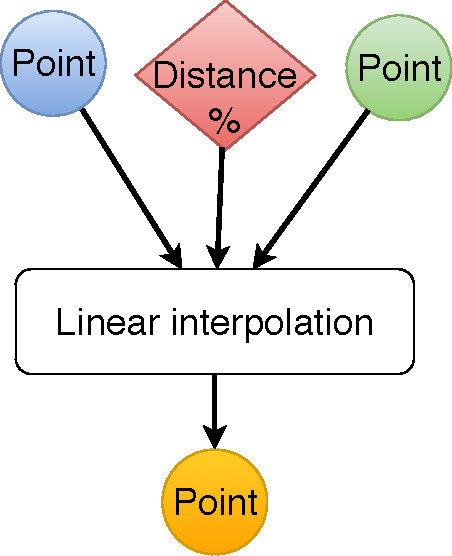
\includegraphics[height=0.3\textwidth]{obrazky-figures/Diagram/Point/DP Navrh operacii-0D - Point Linear interpolation.pdf}}
	\subfloat{
\includegraphics[]{obrazky-figures/Diagram/Draw/1Points/DP Navrh operacii-0D - PointLinearInterpolation.pdf}}
	\caption{Lineárna interpolácia}
	\label{fig:1}
\end{figure}

Ak je zadaná vzdialenosť pomocou dĺžky, použije sa vzorec \ref{eq:LiearnInterpolation}. Pri percentuálnej vzdialenosti sa použije obdobný vzorec, ale vektor medzi bodmi bod1 a bod2 sa nenormalizuje.
\begin{equation}
    bod = bod1 + norm(bod2 - bod1) * vzdialenos\check{t};
	\label{eq:LiearnInterpolation}
\end{equation}


\subsection{Priesečník plochy a úsečky}
http://paulbourke.net/geometry/pointlineplane/

Pri tejto operácii sa používa ľubovolný plošný objekt ako rovina a úsečka ako priamka. Táto geometrická operácia vytvorí bod v mieste, kde sa priamka pretína s rovinou. 


\begin{figure}[H]
	\centering
	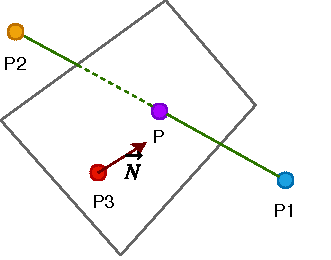
\includegraphics[height=0.3\textwidth]{obrazky-figures/DP Navrh operacii-Intersection.pdf}
	\caption{Pretnutie plochy priamkou}
	\label{fig:1}
\end{figure}


Rovnica pre rovinu, ktorá je tvorená bodom \texttt{P\textsubscript{3}} nachádzajúcom sa na rovine a normálou N, sa dá zapísať ako \ref{eq:rovnicaPlochy_intersection}. 
\begin{equation}
    \textbf{N} \cdot (\textbf{P} - \textbf{P3}) = 0
	\label{eq:rovnicaPlochy_intersection}
\end{equation}

Rovnica pre priamku, ktorá je určená bodmi \texttt{P\textsubscript{1}} a \texttt{P\textsubscript{2}}
\ref{eq:rovnicaPriamky_intersection}
\begin{equation}
	\textup{P}=\textbf{P1}+u (\textbf{P2}-\textbf{P1})
    \label{eq:rovnicaPriamky_intersection}
\end{equation}
	
Bod \texttt{P} označuje priesečník medzi rovinou a priamkou. Pomocou substitúcie získame rovnicu \ref{eq:rovnicaPriesecniku}.

\begin{equation}
	\textbf{N} \cdot (\textbf{P1}+u(\textbf{P2}-\textbf{P1}))) = \textbf{N} \cdot \textbf{P3}
    \label{eq:rovnicaPriesecniku}
\end{equation}

Po vyriešení tejto rovnice dostaneme rovnicu \ref{eq:rovnicaPriesecnikuSolved}. Výslednú pozíciu bodu dostaneme dosadením $u$ do rovnice pre  priamku \ref{eq:rovnicaPriamky_intersection}.
\begin{equation}
	u=\frac
{\textbf{N} \cdot (\textbf{P3}-\textbf{P1})}
{\textbf{N} \cdot (\textbf{P2}-\textbf{P1})}
    \label{eq:rovnicaPriesecnikuSolved}
\end{equation}


\begin{lstlisting}
	Intersection_Plane_Line(string name, Line lineName, Sufrace surfaceName,
	    float visibility)
\end{lstlisting}

Ako je vidieť na obrázku \ref{fig:GraphIntersection_Plane_Line}, pomocou tejto operácie sa vytvorí bod aj mimo zadaných objektov. Problém nastáva, ak je zadaná úsečka paralelná s plochou a teda je kolmá na normálu plochy $N$. Skalárny súčin v menovateli je potom rovný 0. V tomto prípade nieje možné nájsť priesečník.

\begin{figure}[H]
	\centering
	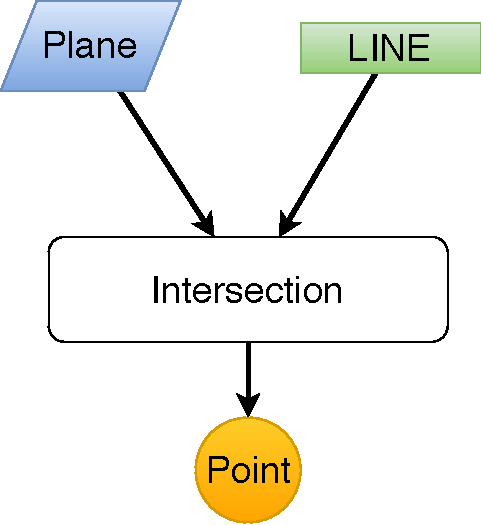
\includegraphics[height=0.3\textwidth]{obrazky-figures/Diagram/Point/DP Navrh operacii-0D - PointIntersection PlaneLine.pdf}
	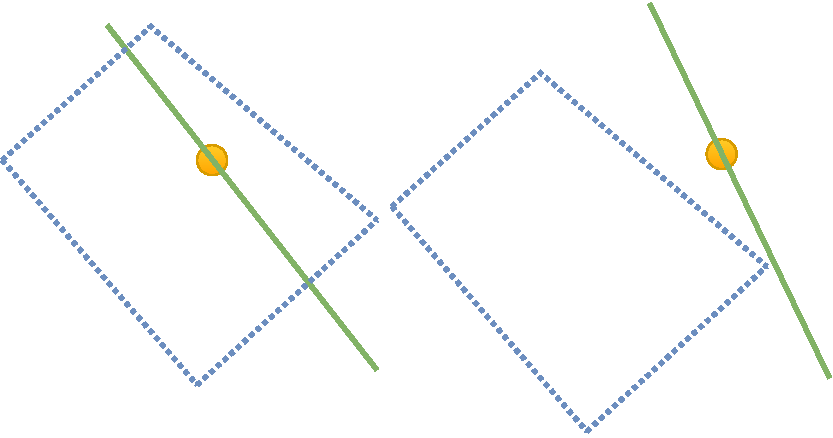
\includegraphics[height=0.3\textwidth]{obrazky-figures/Diagram/Draw/1Points/DP Navrh operacii-0D - PointIntersectionPlaneLine.pdf}
	\caption{Priesečník plochy a priamky.}
	\label{fig:GraphIntersection_Plane_Line}
\end{figure}

\subsection{Stred plochy}
Existuje množstvo možností ako získať stred objektu. Do tejto práce som vybral dve, metódu minimálneho štvorca a priemer všetkých bodov. Pri týchto operáciach sa prevádza 
zadaná plocha z trojrozmerného priestoru  do dvojrozmerného.


\subsubsection{Minimálny štvorec}
Pri tejto operácii sa prejdú všetky body a zistí sa maximálna a minimálna hodnota v jednotlivých osiach a výsledný bod sa nachádza uprostred nich.


\begin{lstlisting}
	SurfaceCenterMinimalSquare(string name, Surface surfaceName, float visibility)
\end{lstlisting}
%//Create point on position of middle of entered surface
%	//	Example:
%	//		SurfaceMiddle(PointName, Circle)	//- Create Point on center of Circle
%	//		SurfaceMiddle(PointName, Rectangle)	//- Create Point on middle of Rectangle
%	//		SurfaceCenter(PointName, Shape)		//- Create Point on middle of shape 
%	//		SurfaceMiddle(PointName, Shape)		//- Create Point on middle of shape - centroid (sum of points / count of points)

\begin{figure}[H]
	\centering
	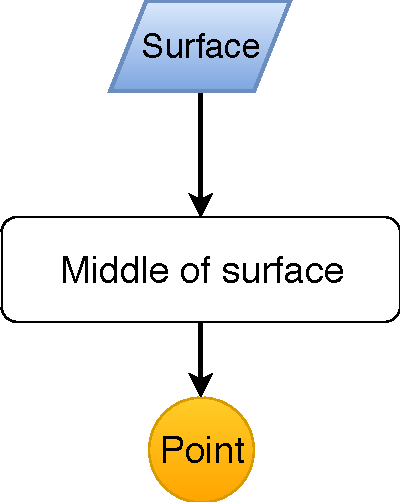
\includegraphics[height=0.3\textwidth]{obrazky-figures/Diagram/Point/DP Navrh operacii-0D - PointMiddle of surface.pdf}
	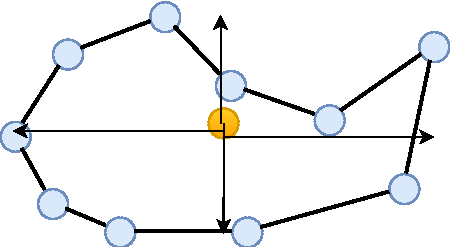
\includegraphics[height=0.3\textwidth]{obrazky-figures/Diagram/Draw/1Points/DP Navrh operacii-0D - PointMiddle of surface.pdf}
	\caption{Stred plochy pomocou minimálneho štvorca }
	\label{fig:1}
\end{figure}



\subsubsection{Priemer všetkých bodov}
Nájde aritmetický priemer všetkých bodov polygónu.

\begin{equation}
    \frac{1}{n} \sum_{i=0}^{n} p_i   
    \label{eq:aritPriemer}
\end{equation}
\begin{lstlisting}
	SurfaceCenterAverage(string name, Surface surfaceName, float visibility)
\end{lstlisting}


\begin{figure}[H]
	\centering
	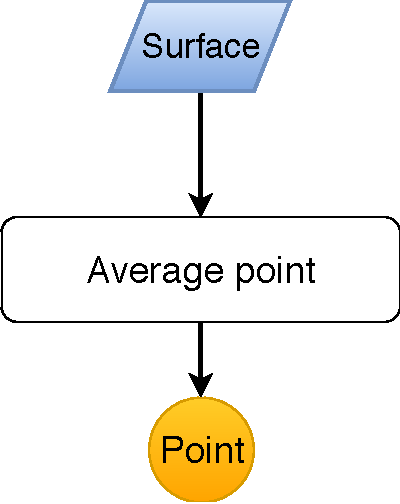
\includegraphics[height=0.3\textwidth]{obrazky-figures/Diagram/Point/DP Navrh operacii-0D - PointCenter of surface.pdf}
	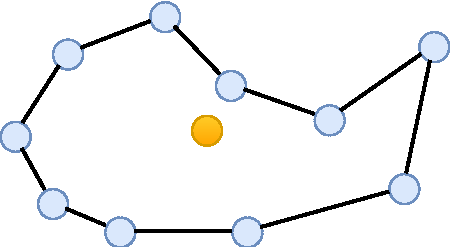
\includegraphics[height=0.3\textwidth]{obrazky-figures/Diagram/Draw/1Points/DP Navrh operacii-0D - PointCenter of surface.pdf}
	\caption{Stred plochy pomocou výpočtu priemeru všetkých bodov}
	\label{fig:1}
\end{figure}

\subsubsection{Stred trojuholníku}
Pre stred trojuholníka existuje v súčastnosti, podľa encyklopédie stredov trojuholníkov, až 30 483 trojuholníkových centier \cite{http://faculty.evansville.edu/ck6/encyclopedia/ETC.html}. Tento počet každým dňom narastá. Pre porovnanie, v decembri 2004 bolo známych 3053 \cite{http://mathworld.wolfram.com/KimberlingCenter.html}. Medzi najznámejšie patria ťažisko (G), ortocentrum (H), stred vpísanej kružnice (I), opísanej kružnice (O) aj stred kružnice deviatich bodov (N). Tieto body sú zaznačené na obrázku \ref{fig:TriangleCenters}.


\begin{figure}[H]
	\centering
	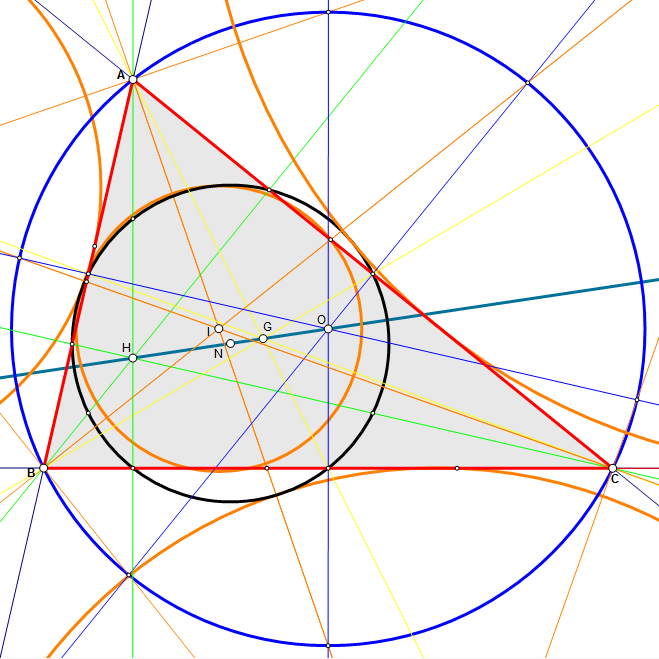
\includegraphics[width=0.9\textwidth]{obrazky-figures/Trigonometric_centres.png}
	\caption{Najznámejšie stredy trojuholníka sú ťažisko (G), ortocentrum (H), stred vpísanej kružnice (I), opísanej kružnice (O) aj stred kružnice deviatich bodov (N)}
	\label{fig:TriangleCenters}
\end{figure}


\paragraph{Ťažisko (Centroid)}\mbox{} \\

Ťažisko trojuholníku sa nachádza v priesečníku troch mediánov trojuholníka. Na nájdenie jeho pozície stačí vypočítať aritmetický priemer vrcholov trojuholníka v jednotlivých osiach \ref{eq:triangleCentroid} \cite{https://brilliant.org/wiki/triangles-centroid/}.



\begin{equation}
    \frac{A+B+C}{3}
    \label{eq:triangleCentroid}
\end{equation}

\paragraph{Stred vpísanej kružnice (Incenter)}\mbox{} \\

Z každého bodu trojuholníka urobíme priamku tak, aby uhly na oboch stranách priam\-ky boli rovnaké. Táto priamka sa nazýva tiež bisektor \cite{https://www.tutorvista.com/math/angle-bisector-theorem}. Stred vpísanej kružnice je na priesečníku týchto priamok.




Stred vpísanej kružnice sa dá vypočítať aj pomocou vzorca \ref{eq:Incenter} \cite{https://www.mathopenref.com/coordincenter.html}.
\begin{equation}
O = \frac{a\ast A+b\ast  B +c \ast C}{a + b + c}
    \label{eq:Incenter}
\end{equation}
kde  $A$, $B$, $C$ sú vrcholy trojuholníka a $a$, $b$, $c$ sú dĺžky strán protiľahlých k vrcholom $A$, $B$, $C$.

\paragraph{Stred opísanej kružnice (Circumcenter)}\mbox{} \\

U jednotlivých strán trojuholníka zistíme stred a z tohoto bodu urobíme kolmice. Kde sa tieto kolmice stretnú, vznikne stred vpísanej kružnice. Veľkosť kružnice je vzdialenosť od stredu k ľubovolnému vrcholu trojuholníka. Táto vzdialenosť je pre všetky vrcholy rovnaká.


\paragraph{Ortocentrum (Orthocenter)}\mbox{} \\

Ortocentrum sa nachádza na priesečníku kolmíc, ktoré prechádzajú cez protiľahlí vrchol. Tieto kolmice sa tiež nazývajú výškou trojuholníka. 
Ak je trojuholník tupý, ortocentrum sa nachádza mimo trojuholníka, ak je trojuholník v niektorom vrchole kolmý, nachádza sa v takomto vrchole aj ortocentrum trojuholníka.

Pre získanie pozície ortocentra zistíme aspoň dve kolmice pomocou operácie \ref{sec:najkratsiauseckaBP}. Pozícia ortocentra sa nachádza v mieste, kde sa tieto kolmice pretínajú. 


\paragraph{Stred kružnice deviatich bodov (NinePointCenter)}\mbox{} \\

Kružnica deviatich bodov, tiež známa ako Feuefbachova kružnica, po nemeckom matematikovi Karl Wilhelm Feuerbach, ktorý ako prvý dokázal, že sa kružnica deviatich bodov dotýka vpísanej a pripísaných kružníc \cite{NinePointTheorem} 


\newtheorem{theorem}{Teorém}
 
\begin{theorem}[{\cite{https://lms.umb.sk/mod/book/tool/print/index.php?id=76930&chapterid=1746} Teorém kružnice deviatich bodov}]
Nech ABC je všeobecný trojuholník, P,Q,R nech sú päty jeho výšok, K,L,M nech sú stredy jeho strán, O nech je priesečník výšok a T,U,V nech sú postupne stredy úsečiek AO,BO,CO. Potom 9 bodov P,Q,R,K,L,M,T,U,V leží na jednej (tzv. Feuerbachovej) kružnici. \todo{Ako citovať? https://lms.umb.sk/mod/book/tool/print/index.php?id=76930&chapterid=1746}

\end{theorem}


\begin{figure}[H]
	\centering
	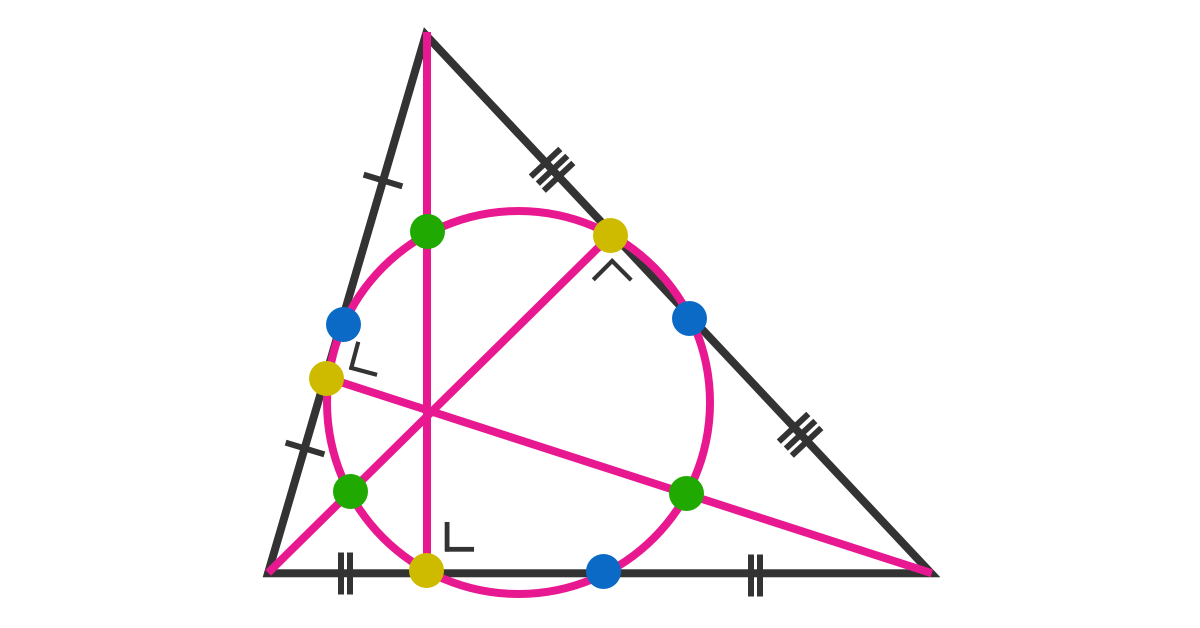
\includegraphics[width=0.9\textwidth]{obrazky-figures/NinePointCircle.png}
	\caption{Kružnica deviatich bodov. Modré body označujú stredy strán, žlté body označujú päty výšok a zelené sú stredy medzi vrcholmi a priesečníkom výšok}
	\label{fig:TriangleCenters}
\end{figure}



\subsection{Stred objektu}
https://www.gamedev.net/forums/topic/468405-center-of-a-3d-object/

Rovnako ako pri 2D objektoch, aj u 3D objektoch je viacero variant získania stredu objektu. Vybral som metódu ohraničujúceho kvádra a metódu priemerného stredu všetkých bodov.


\subsubsection{Stred pomocou ohraničujúceho kvádra}
Prejde všetky body a zoberie maximálnu a minimálnu hodnotu v osiach X, Y a Z. Takto dostaneme ohraničujúci kváder (Bounding box) a ako výsledný bod sa zoberie stred tohoto kvádra.

\begin{lstlisting}
	ObjectCenterBoundingBox(string name, Object3D ObjectName, 
		float visibility)
\end{lstlisting}
		
\begin{figure}[H]
	\centering
	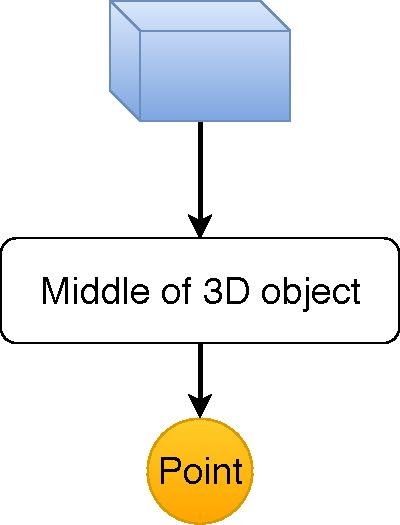
\includegraphics[height=0.3\textwidth]{obrazky-figures/Diagram/Point/DP Navrh operacii-0D - PointMiddle of 3D object.pdf}
	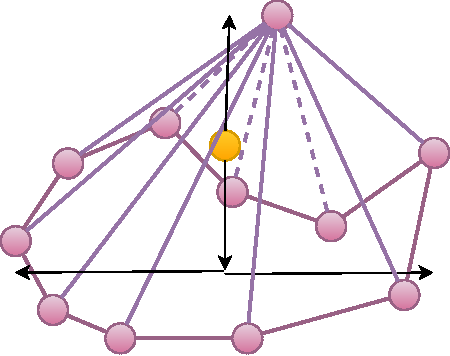
\includegraphics[height=0.3\textwidth]{obrazky-figures/Diagram/Draw/1Points/DP Navrh operacii-0D - PointMiddle of 3D object.pdf}
	\caption{Stred ohraničujúceho kvádra}
	\label{fig:1}
\end{figure}

\subsubsection{Priemer všetkých bodov} 
Pri tejto operácii sa spočítajú koordináty všetkých bodov. To vytvorí tri veľké čísla, ktoré sa následne vydelia počtom bodov.

\begin{lstlisting}
	ObjectCenterAverage(string name, Object3D ObjectName,
		float visibility)
\end{lstlisting}

\begin{figure}[H]
	\centering
	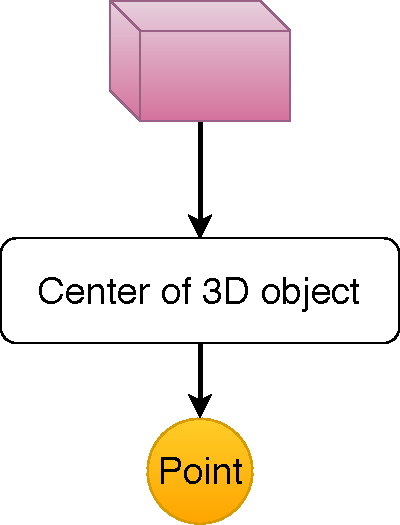
\includegraphics[height=0.3\textwidth]{obrazky-figures/Diagram/Point/DP Navrh operacii-0D - PointCenter of 3D object.pdf}
	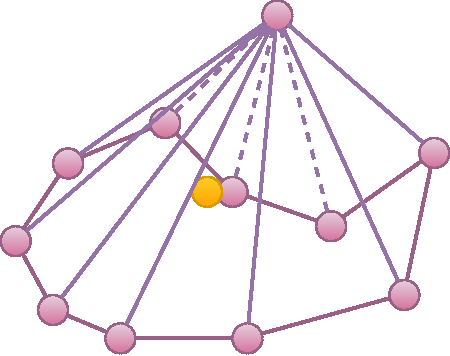
\includegraphics[height=0.3\textwidth]{obrazky-figures/Diagram/Draw/1Points/DP Navrh operacii-0D - PointCenter of 3D object.pdf}
	\caption{Priemerný všetkých bodov}
	\label{fig:1}
\end{figure}

\subsection{Začiatok a koniec úsečky}
Aby sa dalo pristupovať k začiatočnému a koncovému bodu úsečky, vytvoril som operácie \texttt{LineFirstPoint} a \textt{LineSecondPoint}.
\label{sec:begandendofline}

\begin{lstlisting}
    LineFirstPoint(string name, Line lineName, float visibility)
    LineSecondPoint(string name, Line lineName, float visibility)
\end{lstlisting}
		
		


\begin{figure}[H]
	\centering
	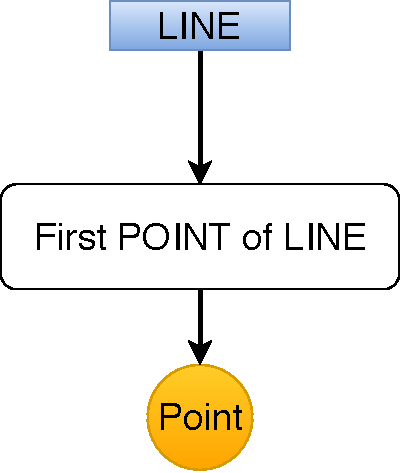
\includegraphics[height=0.3\textwidth]{obrazky-figures/Diagram/Point/DP Navrh operacii-0D - PointFirst POINT of LINE.pdf}
	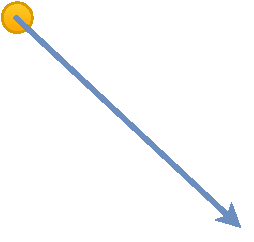
\includegraphics[height=0.3\textwidth]{obrazky-figures/Diagram/Draw/1Points/DP Navrh operacii-0D - PointFirstPointOfLine.pdf}
	\caption{Počiatočný bod úsečky}
	\label{fig:1}
\end{figure}



\begin{figure}[H]
	\centering
	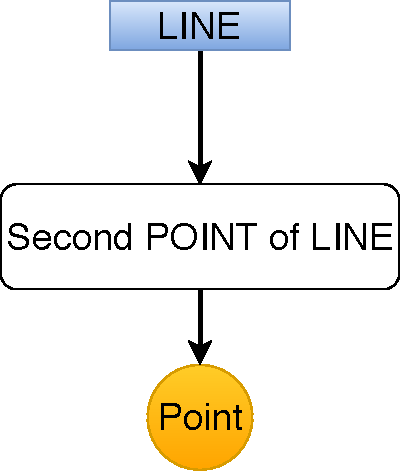
\includegraphics[height=0.3\textwidth]{obrazky-figures/Diagram/Point/DP Navrh operacii-0D - PointSecond POINT of LINE.pdf}
	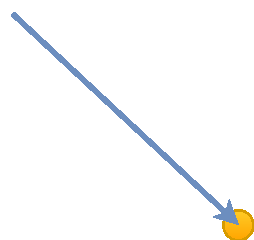
\includegraphics[height=0.3\textwidth]{obrazky-figures/Diagram/Draw/1Points/DP Navrh operacii-0D - PointSecondPointOfLine.pdf}
	\caption{Koncový bod úsečky}
	\label{fig:1}
\end{figure}



	






\section{Úsečkové operácie}
Geometrické operácie vytvárajúce úsečky. 

\subsection{Úsečka}
Úsečka sa nachádza v mnohých operáciach ako parameter, kde zastupuje úlohu smerového vektoru. Každá úsečka sa začína počiatočným bodom a končí koncovým bodom. Pre získanie počiatočného a koncového bodu sú operácie \ref{sec:begandendofline}.

\begin{lstlisting}
	Line(string lineName, Point počiatočný_bod, Point koncový_bod, float visibility)
\end{lstlisting}

\begin{figure}[H]
	\centering
	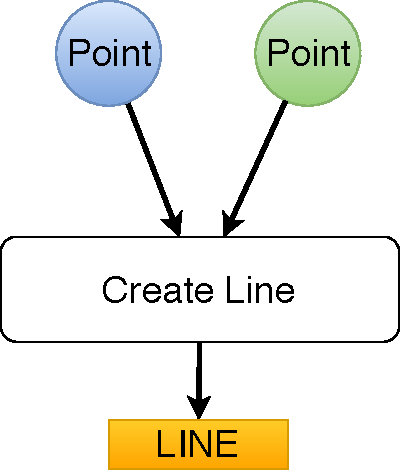
\includegraphics[height=0.3\textwidth]{obrazky-figures/Diagram/Line/DP Navrh operacii-1D - Line.pdf}
	
\includegraphics[]{obrazky-figures/Diagram/Draw/2Line/DP Navrh operacii-1D - Line.pdf}
	\caption{Vytvorenie úsečky pomocou bodu počiatočného a bodu koncového}
	\label{fig:1}
\end{figure}

\subsection{Normalizovanie veľkosti úsečky}
Táto operácia vytvorí úsečku s dĺžkou 1 v rovnakom smere ako pôvodná a s rovnakým počiatočným bodom.
\begin{lstlisting}
	LineNormalize(string lineName, Line l, float visibility)
\end{lstlisting}

\begin{figure}[H]
	\centering
	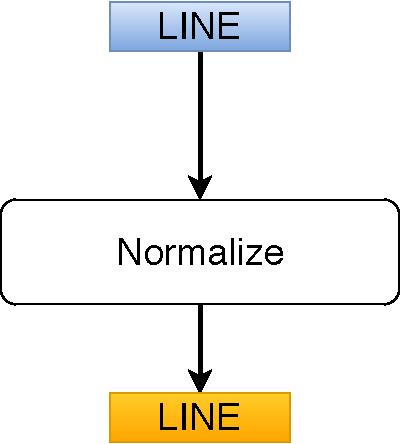
\includegraphics[height=0.3\textwidth]{obrazky-figures/Diagram/Line/DP Navrh operacii-1D - LineNormalize.pdf}
	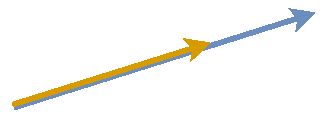
\includegraphics[]{obrazky-figures/Diagram/Draw/2Line/DP Navrh operacii-1D - LineNormalize.pdf}
	\caption{Normalizácia veľkosti úsečky}
	\label{fig:1}
\end{figure}

\subsection{Zmena dĺžky úsečky}
Vytvorenie úsečky so zadanou dĺžkou. Dĺžka môže byť zadaná vzdialenosťou alebo percentuálne od veľkosti zadanej úsečky. Výsledná úsečka je v rovnakom smere a začína v rovnakom bode ako zadaná úsečka.
\begin{lstlisting}
	LineChangeLengthDist(string lineName, Line l, float distance, 
	    float visibility)
	LineChangeLengthPerc(string lineName, Line l, float percent, 
	    float visibility) 
\end{lstlisting}%//percent = (0;100>

\begin{figure}[H]
	\centering
	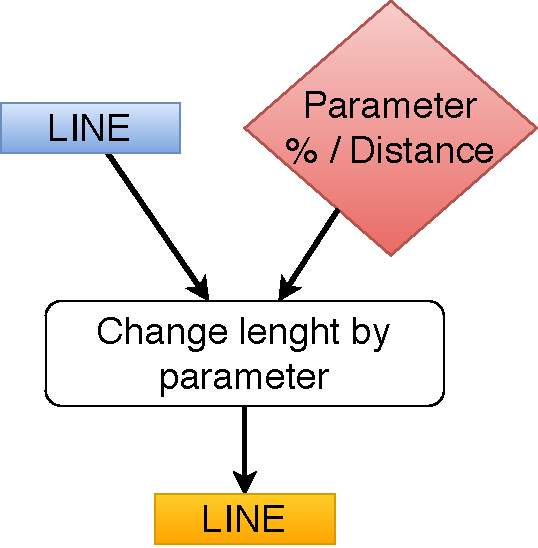
\includegraphics[height=0.3\textwidth]{obrazky-figures/Diagram/Line/DP Navrh operacii-1D - LineChangeLength.pdf}
	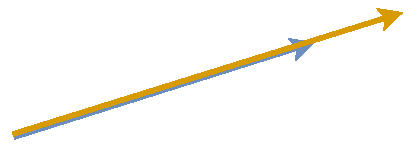
\includegraphics[]{obrazky-figures/Diagram/Draw/2Line/DP Navrh operacii-1D - LineChangeLength.pdf}
	\caption{Zmena veľkosti úsečky}
	\label{fig:1}
\end{figure}

\subsection{Najkratšia úsečka medzi bodom a priamkou}\label{sec:najkratsiauseckaBP}
Priamka je definovaná dvoma bodmi, bodom $P1(x1-y1)$ a bodom $P2(x2,y2)$. 
Rovnica priamky je 
\begin{equation}
    P = P1 + u(P2-P1)
    \label{eq:MinlinePointLine_LineEq}
\end{equation}. 

Na získanie najkratšej vzdialenosti je potrebné nájsť kolmicu od bodu $P3(x3,y3)$ na priamku. Z toho vyplýva, že skalárny súčin medzi nimi musí byť rovný 0, tento vzťah je vidieť v rovnici \ref{eq:MinlinePointLine_LinesEq}.

\begin{equation}
    (P3-P)\cdot(P2-P1) =0 
    \label{eq:MinlinePointLine_LinesEq}
\end{equation}
Bod P označuje najbližší bod na priamke k bodu $P3$.

Substitúciou rovníc \ref{eq:MinlinePointLine_LineEq} a \ref{eq:MinlinePointLine_LinesEq} získame rovnicu \ref{eq:MinlinePointLine_subs}.

\begin{equation}
[P3 - P1 - u(P2-P1)] \cdot (P2 - P1) = 0
    \label{eq:MinlinePointLine_subs}
\end{equation}

Vyriešením tejto rovnice získame rovnicu \ref{eq:MinlinePointLine_subsSolved}, ktorú následne môžeme dosadiť do rovnice pre priamku \ref{eq:MinlinePointLine_LineEq} a získať pozíciu bodu $P$. Ak by sme chceli, aby sa bod vytváral iba na úsečke a nie mimo nej, bolo by potrebné testovať vzdialenosť $u$ na rozmedzie (0,1). Ak je hodnota $u$ záporná alebo väčšia ako jedna,  najbližší bod na priamke k bodu $P3$ sa nachádza mimo zadanej úsečky. 
\begin{equation}
u= \frac
{\left (x3 -x1  \right )\left (x2-x1  \right )
+\left (y3-y1  \right )\left (y2-y1  \right )
+\left (z3-z1  \right )\left (z2-z1  \right )}
{\left \| P2-P1 \right \|^{2}}
    \label{eq:MinlinePointLine_subsSolved}
\end{equation}


Výsledná úsečka je tvorená počiatočným bodom $P$ a koncovým bodom $P3$.
Pre získanie bodu na priamke, ktorý je najbližšie k bodu $P3$ je možné následne použiť operáciu pre získanie počiatočného bodu úsečky \ref{sec:begandendofline}.


\begin{lstlisting}
	MinLineBetweenPointAndLine(string lineName, Point p, Line l,
	float visibility)
\end{lstlisting}

\begin{figure}[H]
	\centering
	\includegraphics[height=0.3\textwidth]{obrazky-figures/Diagram/Line/DP Navrh operacii-1D -  LineMinPL.pdf}
	\includegraphics[height=0.3\textwidth]{obrazky-figures/Diagram/Draw/2Line/DP Navrh operacii-1D -  LineMinPL.pdf}
	\caption{Najkratšia vzdialenosť medzi úsečkou a bodom}
	\label{fig:1}
\end{figure}

\subsection{Najkratšia úsečka medzi dvomi priamkami}
Keďže v trojrozmernom priestore často nenastáva pretnutie dvoch úsečiek práve v jednom bode, je práve najkratšia úsečka medzi dvoma priamkami používaná ako priesečník priamok v trojrozmernom priestore.


Hľadáme najkratšiu úsečku s bodmi $P_a$ a $P_b$, kde $P_a$ leží na priamke definovanou bodmi $P_1$ a $P_2$, a $P_b$ leží na priamke ktorá je definovaná bodmi $P_3$ a $P_4$.

Pre bod $P_a$ môžeme napísať rovnicu  \ref{eq:MinlineLL_Pa}.
\begin{equation}
P_a=P_1 + u_a(P_2-P_1)
    \label{eq:MinlineLL_Pa}
\end{equation}

Podobne pre bod $P_b$ rovnicu \ref{eq:MinlineLL_Pb}.
\begin{equation}
P_b=P_3 + u_b(P_4-P_3)
    \label{eq:MinlineLL_Pb}
\end{equation}

Pri hľadaní najkratšej úsečky medzi týmito priamkami si stačí uvedomiť, že najkratšia úsečka bude na tieto priamky kolmá, čo nám umožňuje zapísať následovné rovnice  \ref{eq:MinlineLL_dotab}.

\begin{equation}
\begin{aligned}
(P_a-P_b) \cdot (P_2-P_1) =0\\
(P_a-P_b) \cdot (P_4-P_3) =0
\end{aligned}
    \label{eq:MinlineLL_dotab}
\end{equation}

Po doplnení  $P_a$ a $P_b$ do týchto rovníc získame rovnice \ref{eq:MinlineLL_dotabExp}.


\begin{equation}
\begin{aligned}
((P_1 + u_a(P_2-P_1))-(P_3 + u_b(P_4-P_3))) \cdot (P_2-P_1) =0\\
((P_1 + u_a(P_2-P_1))-(P_3 + u_b(P_4-P_3))) \cdot (P_4-P_3) =0
\end{aligned}
    \label{eq:MinlineLL_dotabExp}
\end{equation}

Keďže by tieto rovnice boli veľmi rozsiahle, je vhodné si pre riešenie tejto rovnice definovať nasledovnú substitúciu \ref{eq:MinlineLL_subsdmnop}.

\begin{equation}
d_{mnop}=(x_m - x_n)(x_o-x_p)+(y_m - y_n)(y_o-y_p)+(z_m - z_n)(z_o-z_p)
    \label{eq:MinlineLL_subsdmnop}
\end{equation}


Pomocou tejto substitúcie sa dajú rovnice \ref{eq:MinlineLL_dotabExp} zapísať v nasledovne \ref{eq:MinlineLL_dotabExpshort}.


\begin{equation}
\begin{aligned}
d_{1321} + u_a d_{2121} - u_b d_{4321} = 0\\
d_{1343} + u_a d_{2143} - u_b d_{4343} = 0
\end{aligned}
    \label{eq:MinlineLL_dotabExpshort}
\end{equation}

Vyriešením týchto rovníc pre $u_a$ získame rovnicu \ref{eq:MinlineLL_dotabExpshortSolving}.
\begin{equation}
 u_a= \frac
 {d_{1343} d_{4321} - d_{1321} d_{4343} }
 {d_{2121} d_{4343} - d_{2143} d_{2143} }
    \label{eq:MinlineLL_dotabExpshortSolving}
\end{equation}

Keď už poznáme $u_a$, pomocou dosadenia do rovnice \ref{eq:MinlineLL_dotabExpshortSolved_ub} získame $u_b$ 

\begin{equation}
\begin{aligned}
u_b  = \frac{d_{1321} + u_a d_{2121}}{d_{4321}}
\end{aligned}
    \label{eq:MinlineLL_dotabExpshortSolved_ub}
\end{equation}


http://paulbourke.net/geometry/pointlineplane/
\begin{lstlisting}
	MinLineBetweenLineAndLine(string lineName, Line l1, Line l2, float visibility)
\end{lstlisting}

\begin{figure}[H]
	\centering
	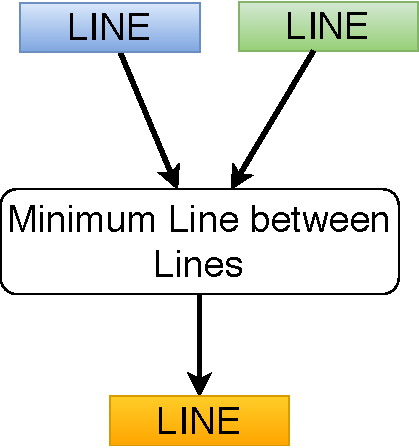
\includegraphics[height=0.3\textwidth]{obrazky-figures/Diagram/Line/DP Navrh operacii-1D - LineMinLL.pdf}
	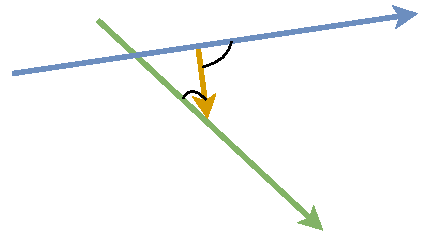
\includegraphics[height=0.3\textwidth]{obrazky-figures/Diagram/Draw/2Line/DP Navrh operacii-1D - LineMinLL.pdf}
	\caption{Najkratšia vzdialenosť medzi dvomi úsečkami}
	\label{fig:1}
\end{figure}


\subsection{Najkratšia úsečka medzi plochou a bodom}
http://paulbourke.net/geometry/pointlineplane/


Rovina je definovaná pomocou normáli $\overrightarrow{N}=(A, B, C)$ a bodom na nej ležiacom $P_a=(x_a,y_a,z_a)$.
Hľadaná úsečka má rovnaký smer ako normála plochy.
Vzdialenosť medzi touto rovinou a bodom $P_b=(x_b,y_b,z_b)$ dostaneme pomocou vzorca \ref{eq:minlineSP}, kde premietneme vektor medzi bodom $P_b$ a bodom $P_a$ na normálu roviny $\overrightarrow{N}$ pomocou skalárneho súčinu. 
\begin{equation}
 distance = (P_b - P_a) \cdot \overrightarrow{N}
    \label{eq:minlineSP}
\end{equation}

Bod $P$ získame vynásobením vektora $\overrightarrow{N}$ touto vzdialenosťou a následným odčítaním od bodu $P_b$ \ref{eq:minlineSP_P}.
\begin{equation}
 P = P_b - (\overrightarrow{N} * distance)
    \label{eq:minlineSP_P}
\end{equation}

Výsledná úsečka má počiatočný bod na ploche a koncový bod $P_b$ 

%Každý bod $P=(x,y,z)$ leží na rovine, ak splňuje \ref{eq:rovnicaPlochySP}.
%\begin{equation}
%Ax+By+Cz+D = 0
%    \label{eq:rovnicaPlochySP}
%\end{equation}




\begin{lstlisting}
	MinLineBetweenPointAndSurface(string lineName, Point p, Surface s,
	    float visibility)
\end{lstlisting}

\begin{figure}[H]
	\centering
	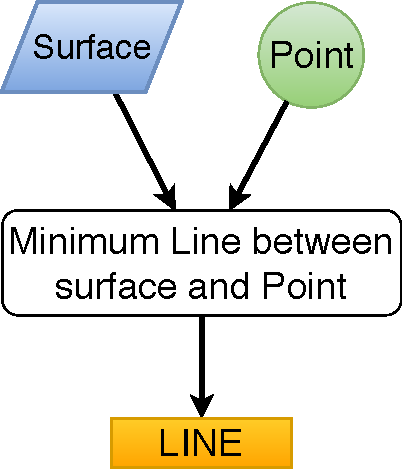
\includegraphics[height=0.3\textwidth]{obrazky-figures/Diagram/Line/DP Navrh operacii-1D - LineMinSP.pdf}
	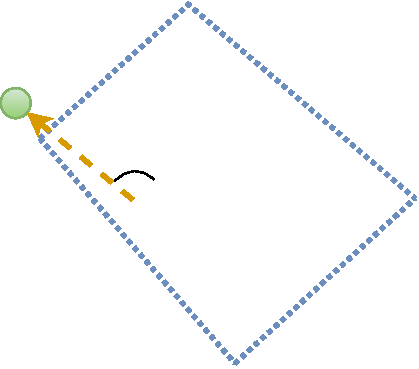
\includegraphics[height=0.3\textwidth]{obrazky-figures/Diagram/Draw/2Line/DP Navrh operacii-1D - LineMinSP.pdf}
	\caption{Najkratšia vzdialenosť medzi plochou a bodom}
	\label{fig:1}
\end{figure}


\subsection{Najkratšia úsečka}
Aby bolo možné jednoduchšie pristupovať k predchádzajúcim operáciam, vytvoril som pre ne aj alternatívny zápis, ktorý identifikuje aké parametre dostal a podľa nich zvolí pomocou ktorej operácie má riešiť, teda najkratšia úsečka medzi bodom a priamkou, bodom a plochou alebo dvomi priamkami.

\begin{lstlisting}
	MinLine(string lineName, Line l, Point p, float visibility)
	MinLine(string lineName, Line l1, Line l2, float visibility)
	MinLine(string lineName, Surface s, point p, float visibility)
\end{lstlisting}




\subsection{Vektorový súčin}\label{subsec:crossproduct}
Vytvára úsečku, ktorá je kolmá na zadané úsečky (priamky). Zadané úsečky sa najprv prevedú na vektory ($koncov\acute{y}\_bod - za\check{c}iato\check{c}n\acute{y}\_bod$).
Veľkosť úsečky závisí od veľkosti zadaných úsečiek a od uhla ktorý zvierajú. 

\begin{equation}
 L_1 \times L_2 =  \{
 y_{l1} z_{l2} + y_{l2} z_{l1} ,
 z_{l1} x_{l2} + z_{l2} x_{l1} ,
 x_{l1} y_{l2} + x_{l2} y_{l1}\}
    \label{eq:cross}
\end{equation}


\begin{lstlisting}
	CrossProduct(string lineName, Line l1, Line l2, float visibility)
\end{lstlisting}

\begin{figure}[H]
	\centering
	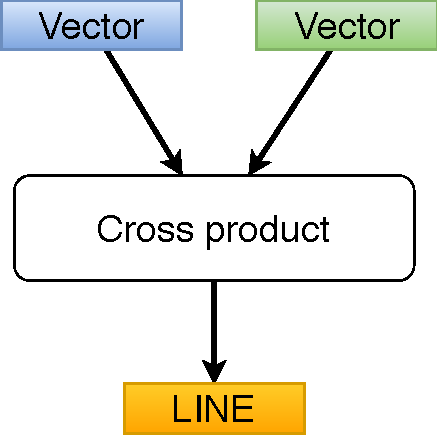
\includegraphics[height=0.3\textwidth]{obrazky-figures/Diagram/Line/DP Navrh operacii-1D - LineCross.pdf}
	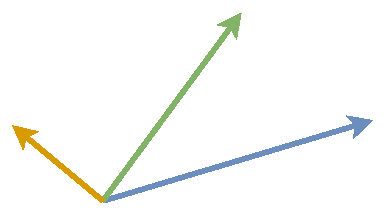
\includegraphics[height=0.3\textwidth]{obrazky-figures/Diagram/Draw/2Line/DP Navrh operacii-1D - LineCross.pdf}
	\caption{Vektorový súčin}
	\label{fig:1}
\end{figure}

\subsection{Normála roviny}
Normála plochy sa pri väčšine plošných objektov predvypočítava už pri vytváraní. Ak objekt nebol vytváraný už priamo so zadanou normálou, je potrebné ju vypočítať. Výpočet normály sa robí pomocou vektorového súčinu \ref{subsec:crossproduct}, ktorého výsledný vektor je potrebné normalizovať, teda vydeliť jeho dĺžkou.


\begin{lstlisting}
	SurfaceNormal(string lineName, Surface s, float visibility)
\end{lstlisting}


\begin{figure}[H]
	\centering
	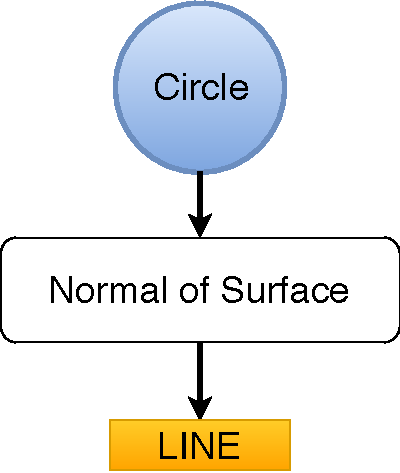
\includegraphics[height=0.3\textwidth]{obrazky-figures/Diagram/Line/DP Navrh operacii-1D - LineSurfaceNormal.pdf}
	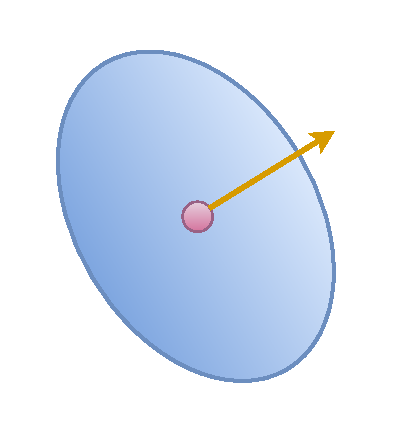
\includegraphics[height=0.3\textwidth]{obrazky-figures/Diagram/Draw/2Line/DP Navrh operacii-1D - LineSurfaceNormal.pdf}
	\caption{Normála roviny}
	\label{fig:1}
\end{figure}



\subsection{Presun úsečky}
Táto operácia nepremiestňuje zadanú úsečku ale vytvára úsečku v rovnakom smere a rovnakej dĺžke ako zadaná úsečka $L$, ale počiatočný bod bude na pozícii zadaného bodu $P$. 
Koncový bod úsečky $P2$ získame pomocou vzorca \ref{eq:LineReloc}. 

\begin{equation}
    P2 = P + (P_{2L}-P_{1L})
    \label{eq:LineReloc}
\end{equation}


\begin{lstlisting}
	LineRelocationByPoint(string lineName, Line l, Point p, float visibility)
\end{lstlisting}


\begin{figure}[H]
	\centering
	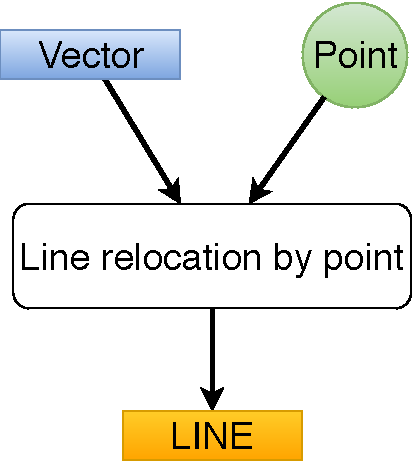
\includegraphics[height=0.3\textwidth]{obrazky-figures/Diagram/Line/DP Navrh operacii-1D - LineRelocation.pdf}
	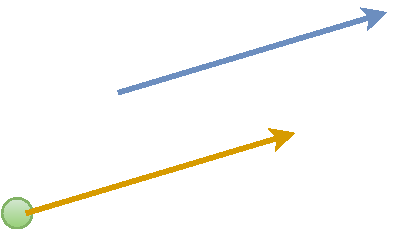
\includegraphics[height=0.3\textwidth]{obrazky-figures/Diagram/Draw/2Line/DP Navrh operacii-1D - LineRelocation.pdf}
	\caption{Presun úsečky}
	\label{fig:1}
\end{figure}






\section{Plošné operácie}


\subsection{Obdĺžnik z úsečky}


\begin{lstlisting}
	RectangleFromLine(string surfaceName, Line l, float width,
	    Point surfacePoint, short type, float visibility)
	RectangleFromLine(string surfaceName, Line l, float width,
	    Vector3 normalVector, short type, float visibility)
\end{lstlisting}
%//create Rectangle from Line l
%/*type:
%	0 - width/2 to left, width/2 to right
%	1 - width to left
%	2 - width to right
%	*/
%	//if normal vector is not perpendicular to line, as normal is used normalized dot product %between line and normal vector
%	//if normal vector is same direction as line normal, exception occure
%	//If surface point is not on line l, exception occure

\begin{figure}[H]
	\centering
	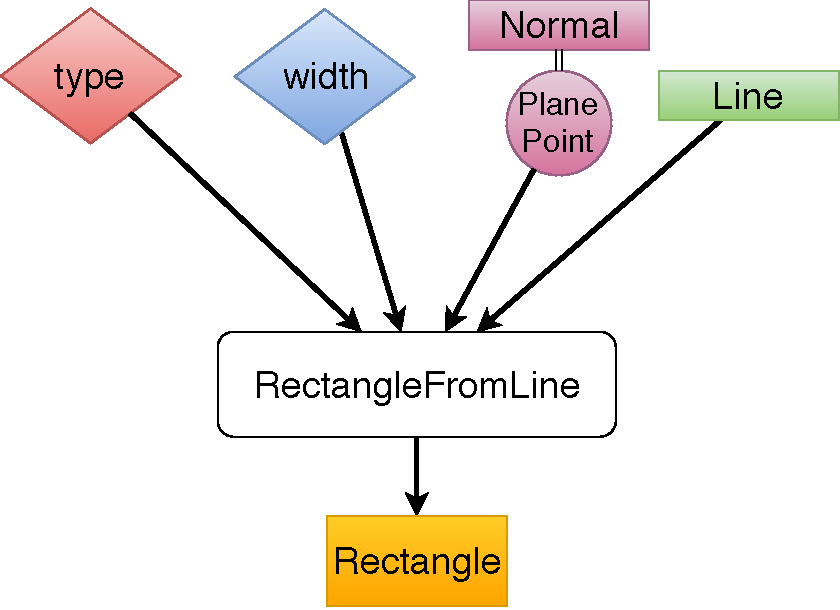
\includegraphics[height=0.3\textwidth]{obrazky-figures/Diagram/Surface/DP Navrh operacii-2D - SurfaceRectangleFromLine.pdf}
	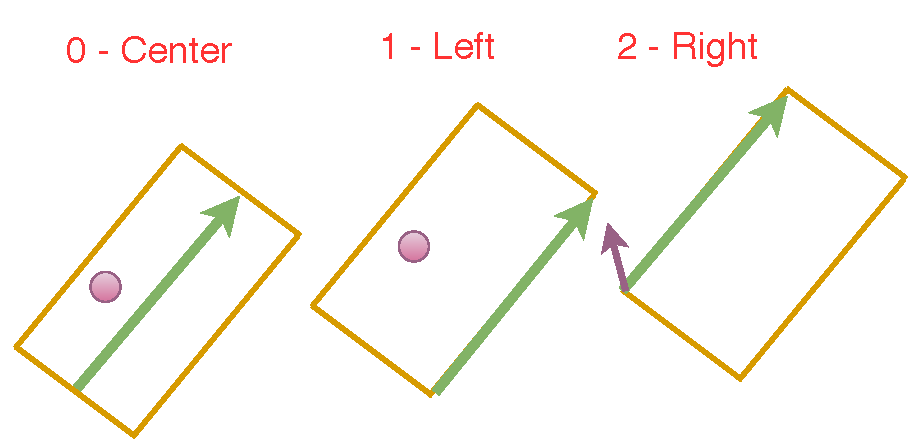
\includegraphics[height=0.3\textwidth]{obrazky-figures/Diagram/Draw/3Plane/DP Navrh operacii-2D - SurfaceRectangleFromLine.pdf}
	\caption{Vytvorenie obdĺžnika pomocou úsečky.}
	\label{fig:1}
\end{figure}

\subsection{Kruh}
\begin{lstlisting}
	Circle(string surfaceName, Point center, float radius, Line lineNormal,
	    float visibility)
	Circle(string surfaceName, Point center, Point outlinePoint,
	    Point planePoint, float visibility)
\end{lstlisting}

\begin{figure}[H]
	\centering
	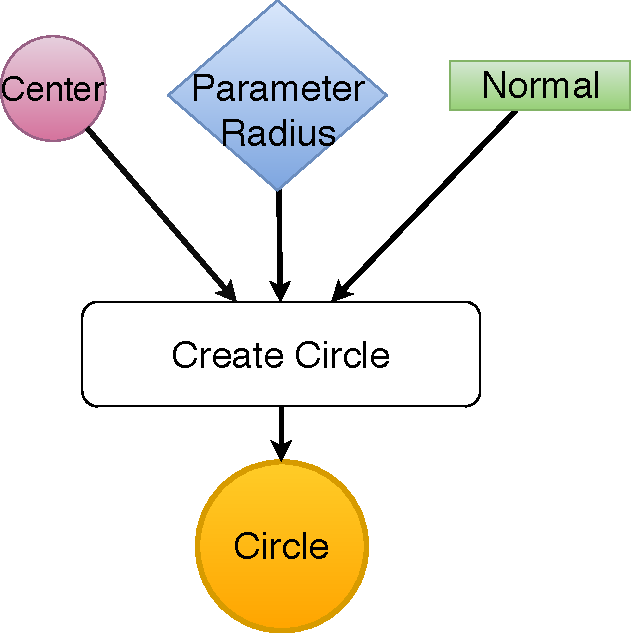
\includegraphics[height=0.3\textwidth]{obrazky-figures/Diagram/Surface/DP Navrh operacii-2D - SurfaceCreate Circle.pdf}
	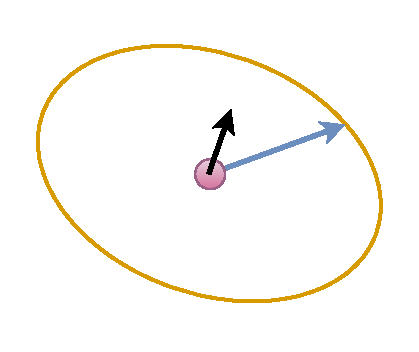
\includegraphics[height=0.3\textwidth]{obrazky-figures/Diagram/Draw/3Plane/DP Navrh operacii-2D - SurfaceCreate Circle.pdf}
	\caption{Kruh pomocou priemeru a normály}
	\label{fig:1}
\end{figure}

\begin{figure}[H]
	\centering
	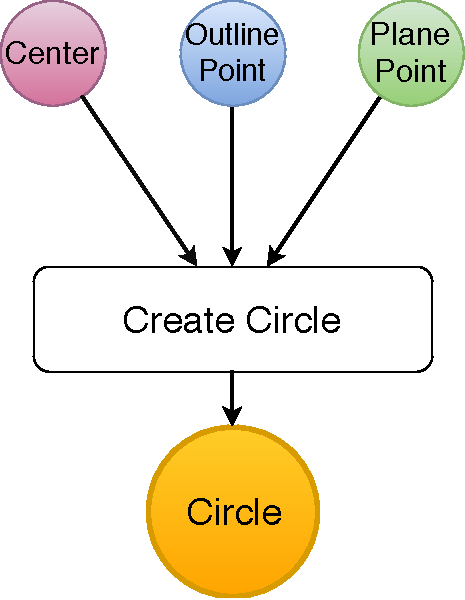
\includegraphics[height=0.3\textwidth]{obrazky-figures/Diagram/Surface/DP Navrh operacii-2D - SurfaceCreate Circle2.pdf}
	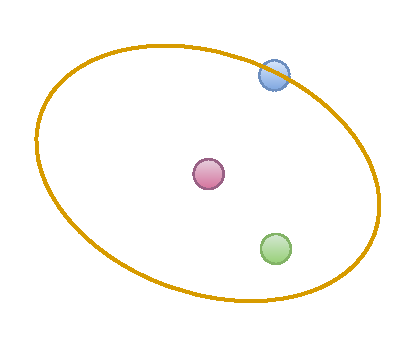
\includegraphics[height=0.3\textwidth]{obrazky-figures/Diagram/Draw/3Plane/DP Navrh operacii-2D - SurfaceCreate Circle2.pdf}
	\caption{Kruh vytvorený troma bodmi, kde jeden bod udáva stred a pomocou ďalších dvoch bodov sa určí priemer a smer normály}
	\label{fig:1}
\end{figure}


\subsection{Trojuholník}
\begin{lstlisting}
	Triangle(string surfaceName, Line l, Point p, float visibility)
	Triangle(string surfaceName, Point p1, Point p2, Point p3, float visibility)
\end{lstlisting}

\begin{figure}[H]
	\centering
	\includegraphics[height=0.3\textwidth]{obrazky-figures/Diagram/Surface/DP Navrh operacii-2D - SurfaceTriangle.pdf}
	\includegraphics[height=0.3\textwidth]{obrazky-figures/Diagram/Draw/3Plane/DP Navrh operacii-2D - SurfaceCreate Triangle.pdf}
	\caption{Trojuholník}
	\label{fig:1}
\end{figure}


\subsection{Obdĺžnik}
\begin{lstlisting}
	Rectangle(string surfaceName, Point center, float X, float Y, float Roll/*[0,360]*/, Line normal, float visibility)
\end{lstlisting}
\begin{figure}[H]
	\centering
	\includegraphics[height=0.3\textwidth]{obrazky-figures/Diagram/Surface/DP Navrh operacii-2D - SurfaceCreate Rectangle.pdf}
	\includegraphics[height=0.3\textwidth]{obrazky-figures/Diagram/Draw/3Plane/DP Navrh operacii-2D - SurfaceCreate Rectangle.pdf}
	\caption{Obdĺžnik}
	\label{fig:1}
\end{figure}


\subsection{Shape}
Táto operácia má ako jediná premenlivý počet bodov.
\begin{lstlisting}
	Shape(string surfaceName, Point p1, Point p2, Point p3, ..., float visibility)//minimum 3 points
\end{lstlisting} 

\begin{figure}[H]
	\centering
	\includegraphics[height=0.3\textwidth]{obrazky-figures/Diagram/Surface/DP Navrh operacii-2D - SurfaceCreate Shape.pdf}
	\includegraphics[height=0.3\textwidth]{obrazky-figures/Diagram/Draw/3Plane/DP Navrh operacii-2D - SurfaceCreate Shape.pdf}
	\caption{Shape}
	\label{fig:1}
\end{figure}



\subsection{Opísaná kružnica}
\begin{lstlisting}
	Circumscribed(string surfaceName, Triangle t, float visibility)
\end{lstlisting} 

\begin{figure}[H]
	\centering
	\includegraphics[height=0.3\textwidth]{obrazky-figures/Diagram/Surface/DP Navrh operacii-2D - SurfaceCircumscribed Circle.pdf}
	\includegraphics[height=0.3\textwidth]{obrazky-figures/Diagram/Draw/3Plane/DP Navrh operacii-2D - SurfaceCircumscribed Circle.pdf}
	\caption{Opísaná kružnica}
	\label{fig:1}
\end{figure}

\subsection{Vpísaná kružnica}
\begin{lstlisting}
	Inscribed(string surfaceName, Triangle t, float visibility)
\end{lstlisting}	

\begin{figure}[H]
	\centering
	\includegraphics[height=0.3\textwidth]{obrazky-figures/Diagram/Surface/DP Navrh operacii-2D - SurfaceInscribed Circle.pdf}
	\includegraphics[height=0.3\textwidth]{obrazky-figures/Diagram/Draw/3Plane/DP Navrh operacii-2D - SurfaceInscribed Circle.pdf}
	\caption{Vpísaná kružnica}
	\label{fig:1}
\end{figure}







\section{Priestorové operácie}
Tieto operácie sú zatiaľ len koncepty a teda nie sú implementované.

\subsection{Pyramida}
\begin{lstlisting}
    Pyramid(string objectName, Surface s, float distance, float visibility) //Create Pyramid by     distance from center
    Pyramid(string objectName, Surface s, Point p, float visibility) //Create Pyramid by Point
\end{lstlisting}

\begin{figure}[H]
	\centering
	\includegraphics[height=0.3\textwidth]{obrazky-figures/Diagram/Volumetric/DP Navrh operacii-3D - ObjectsCreate Pyramid by distance from center.pdf}
	\includegraphics[height=0.3\textwidth]{obrazky-figures/Diagram/Draw/4Object/DP Navrh operacii-3D - ObjectsCreate Pyramid by distance from center.pdf}
	\caption{text}
	\label{fig:1}
\end{figure}

\begin{figure}[H]
	\centering
	\includegraphics[height=0.3\textwidth]{obrazky-figures/Diagram/Volumetric/DP Navrh operacii-3D - ObjectsCreate Pyramid.pdf}
	\includegraphics[height=0.3\textwidth]{obrazky-figures/Diagram/Draw/4Object/DP Navrh operacii-3D - ObjectsCreate Pyramid.pdf}
	\caption{text}
	\label{fig:1}
\end{figure}


\subsection{Extrudovanie} 
Natiahne plochu do priestoru v smere normály. 
\begin{lstlisting}
    Extrude(string objectName, Surface s, float distance, float visibility) 
\end{lstlisting}

\begin{figure}[H]
	\centering
	\includegraphics[height=0.3\textwidth]{obrazky-figures/Diagram/Volumetric/DP Navrh operacii-3D - ObjectsExtrude.pdf}
	\includegraphics[height=0.3\textwidth]{obrazky-figures/Diagram/Draw/4Object/DP Navrh operacii-3D - ObjectsExtrude.pdf}
	\caption{Extrudovanie}
	\label{fig:1}
\end{figure}


\subsection{Zagulatená plocha}
\begin{lstlisting}
    SpericalCurvedSurface(string objectName, Surface s, float distance, float visibility)
\end{lstlisting}

\begin{figure}[H]
	\centering
	\includegraphics[height=0.3\textwidth]{obrazky-figures/Diagram/Volumetric/DP Navrh operacii-3D - ObjectsSpherical curved surface.pdf}
	\includegraphics[height=0.3\textwidth]{obrazky-figures/Diagram/Draw/4Object/DP Navrh operacii-3D - ObjectsSpherical curved surface.pdf}
	\caption{Zagulatenie plochy}
	\label{fig:1}
\end{figure}



\subsection{Valec}
\begin{lstlisting}
Cylinder(string objectName, Line l, float radius, float visibility)
\end{lstlisting}

\begin{figure}[H]
	\centering
	\includegraphics[height=0.3\textwidth]{obrazky-figures/Diagram/Volumetric/DP Navrh operacii-3D - ObjectsCylinder.pdf}
	\includegraphics[height=0.3\textwidth]{obrazky-figures/Diagram/Draw/4Object/DP Navrh operacii-3D - ObjectsCylinder.pdf}
	\caption{Valec}
	\label{fig:1}
\end{figure}




\chapter{Grafické rozhranie}
Okrem programátorského rozhrania, som vytvoril aj jednoduché grafické užívateľské rozhranie pomocou knižnice QT. Toto grafické rozhranie umožňuje užívateľovi jednoduchšiu správu tvorby geometrických objektov a to aj vďaka prehľadnému zoznamu použitých geometrických operácii a zoznamu referencovaných premenných. 

\section{Zoznam geometrických operácii}
Aby bolo jednoduchšie vytvárať objekty, grafické rozhranie umožňuje geometrické operácie pridať, upraviť, mazať a aj vložiť na ľubovoľné miesto. Tieto operácie je tiež možné ľubovolne presúvať. Keďže parametre operácii môžu odkazovať iba na predchádzajúce objekty, je nutné pri upravovaní, presúvaní a mazaní tieto parametre kontrolovať. Grafické rozhranie následne zobrazí, u ktorých operácii sa nachádzajú nevyhovujúce parametre a tieto objekty (a objekty na nich závislé) sa nebudú vykresľovať.

\todo{Zobrazenie grafického rozhrania}


\subsection{Pridanie, vloženie a úprava geometrických operácii} 
Dialógové okno umožňuje výber operácie,  ktorá sa má použiť, zo zoznamu geometrických operácii. V zozname sa nachádza názov geometrickej operácie, parametre ktoré operácia potrebuje a nápoveda, ktorá informuje užívateľa čo daná operácia robí.
Po vybraní operácie zo zoznamu, sa zobrazia v pravej časti dialógového okna parametre vybranej operácie. Ak je dialógové okno v režime úpravy (okno sa zobrazilo po dvojkliku na zozname geometrických operácii), sú pri vybraní rovnakého typu operácie tieto parametre už predvyplnené hodnotami zvolenej operácie na úpravu.

Ako prvý parameter je názov takto vytvoreného objektu, ktorý je pri novo vytváraných objektoch (režim okna pridanie alebo vloženie) predvyplnený, ale je možné ho upraviť na ľubovolnú hodnotu.  
Po názve objektu nasleduje viditeľnosť objektu, ktorá určuje, ako bude takto vytvorený objekt viditeľný. Pri hodnote viditeľnosti $\leq0$ je objekt neviditeľný a pri hodnote $\geq1$ je objekt plne viditeľný. Ak je táto hodnota v rozmedzí (0-1) je tento objekt priehľadný. 
Ďalej nasledujú samotné parametre operácie typu $Float,  Point, Line, Surface$ a ďalšie. Parametrom typu $Float$ sa dá nastaviť názov, podľa ktorého sa na ne bude odkazovať. Tento názov ale nieje povinný a pre nereferencované parametre stačí nechať políčko prázdne. Parametre typu $Float$, ktoré sú týmto názvom pomenované, sa následne zobrazia aj v zozname referencovaných parametrov.
V poslednom stĺpci sa nachádza nápoveda k danému parametru.

Po zadaní hodnoty sa overuje, či je táto hodnota valídna pre daný parameter. To zahŕňa testovanie, či hodnota zadaná parametru $Float$ je desatinné číslo a pri ostatných parametroch sa testuje, či existuje objekt s rovnakým názvom ako bol zadaný a či je tento objekt správnym typom prípadne podtypom (viac o typoch objektov v kapitole  \ref{chapt:Geometrické_tvary}). Tiež sa testuje aj názov objektu a názov referencovaného parametra na unikátnosť.
Ak hodnota parametra nesplňuje niektorú požiadavku, je toto políčko označené červenou farbou pozadia, čo upozorňuje užívateľa na chybu. Ak je hodnota valídna, políčko sa označí zeleným pozadím. Prázdne políčko je označené bielim pozadím. 

\begin{figure}[hbt]
	\centering
	\includegraphics[width=1\textwidth]{obrazky-figures/Dialog.png}
	\caption{Dialógové okno na pridanie, vloženie a úpravu operácii. Ukážka úpravy bodu s názvom $p3$ s jednou chybne zadanou hodnotou }
	\label{fig:dialogWindow}
\end{figure}

\chapter{Záver}

\section{Logické operácie nad objemovými telesami}
Vo výsledku by sa malo dať vytvárať nad objektami logické operácie ako zjednotenie (union), prienik (intersection) a rozdiel medzi množinami (minus). Keďže sú tieto operácie náročné na spracovanie, rozhodol som sa využiť niektorú z voľne dostupných knižníc. Našiel som niekoľko dostupných knižníc, ktoré by sa dali použiť. Jednou z nich je \texttt{libigl}\cite{libigl} ale na integráciu do aplikácie zatiaľ nie sú dostatočne spracované objemové objekty.
%https://stackoverflow.com/questions/24694845/c-library-for-mesh-to-mesh-intersection-what-is-available
%https://libigl.github.io/tutorial/#boolean-operations-on-meshes

libigl je používaná aj veľkými spoločnosťami ako je Activision, EA, Adobe, Google, Epic Games, Microsoft, Pixar, UBISOFT a ďalšie. Táto knižnica je distribuovaná pod licenciou Mozilla Public License (MPL).
Obľúbená je hlavne pre svoju jednoduchosť. Tvorba boolovských operácii nad mesh stačí zavolať funkciu: 

\begin{lstlisting}
igl::copyleft::cgal::mesh_boolean(VA,FA,VB,FB,MESH_BOOLEAN_TYPE_UNION,VC,FC);
\end{lstlisting}


\section{Použitie parametru z iného objektu}
Je potrebné navrhnúť, na ktoré hodnoty u objektoch sa bude dať odkazovať. 

\section{Pridanie vykreslovania orientovaného grafu pomocou knižnice GraphViz}

\todo{ukážka kde sa má tento graf vykresliť a ako bude vyzerat}

\section{Vykreslovanie objektov v grafickom rozhraní pomocou QOpenGLWidget}

\section{Pridanie textúry na objekt}
Po dvojkliku v zozname objektov by sa mala otvoriť ponuka pre nahratie textúry a ďalšie úpravy
